%-------------------------
% Presentacion: Clasificacion de Digitos MNIST con MLP
% Para Overleaf (pdflatex) — max 5 minutos
%-------------------------
% INSTRUCCIONES PARA OVERLEAF:
%   1. Sube este .tex y TODOS los .png de la carpeta resultados/
%   2. Pon los .png en la misma carpeta que el .tex (o en resultados/)
%   3. Compila con pdflatex
%-------------------------

\documentclass[aspectratio=169]{beamer}

\usetheme{Madrid}
\usecolortheme{seahorse}
\setbeamertemplate{navigation symbols}{}
\setbeamertemplate{footline}[frame number]

\usepackage[utf8]{inputenc}
\usepackage[T1]{fontenc}
\usepackage[spanish]{babel}
\usepackage{graphicx}
\usepackage{booktabs}
\usepackage{amsmath}

% Ruta a las imagenes — ajusta si las pones en subcarpeta
\graphicspath{{../resultados/}{resultados/}{./}}

% Title info - EDITA ESTOS CAMPOS
\title[MNIST MLP]{Clasificacion de Digitos Escritos a Mano con MLP}
\subtitle{Dataset MNIST + Imagenes Propias}
\author{Tu Nombre Aqui}
\institute{Introduccion a Machine Learning}
\date{\today}

\begin{document}

%========== SLIDE 1: TITULO ==========
\begin{frame}
\titlepage
\end{frame}

%========== SLIDE 2: PROBLEMA ==========
\begin{frame}{El Problema}
\begin{columns}
\column{0.55\textwidth}
\begin{itemize}
    \item \textbf{Objetivo:} Clasificar digitos escritos a mano (0--9)
    \item \textbf{Dataset:} MNIST --- 70,000 imagenes
    \begin{itemize}
        \item 60,000 entrenamiento
        \item 10,000 prueba
    \end{itemize}
    \item \textbf{Formato:} 28$\times$28 pixeles, escala de grises
    \item \textbf{Reto adicional:} Probar con 62 imagenes propias dibujadas a mano en papel
\end{itemize}

\column{0.4\textwidth}
\begin{center}
    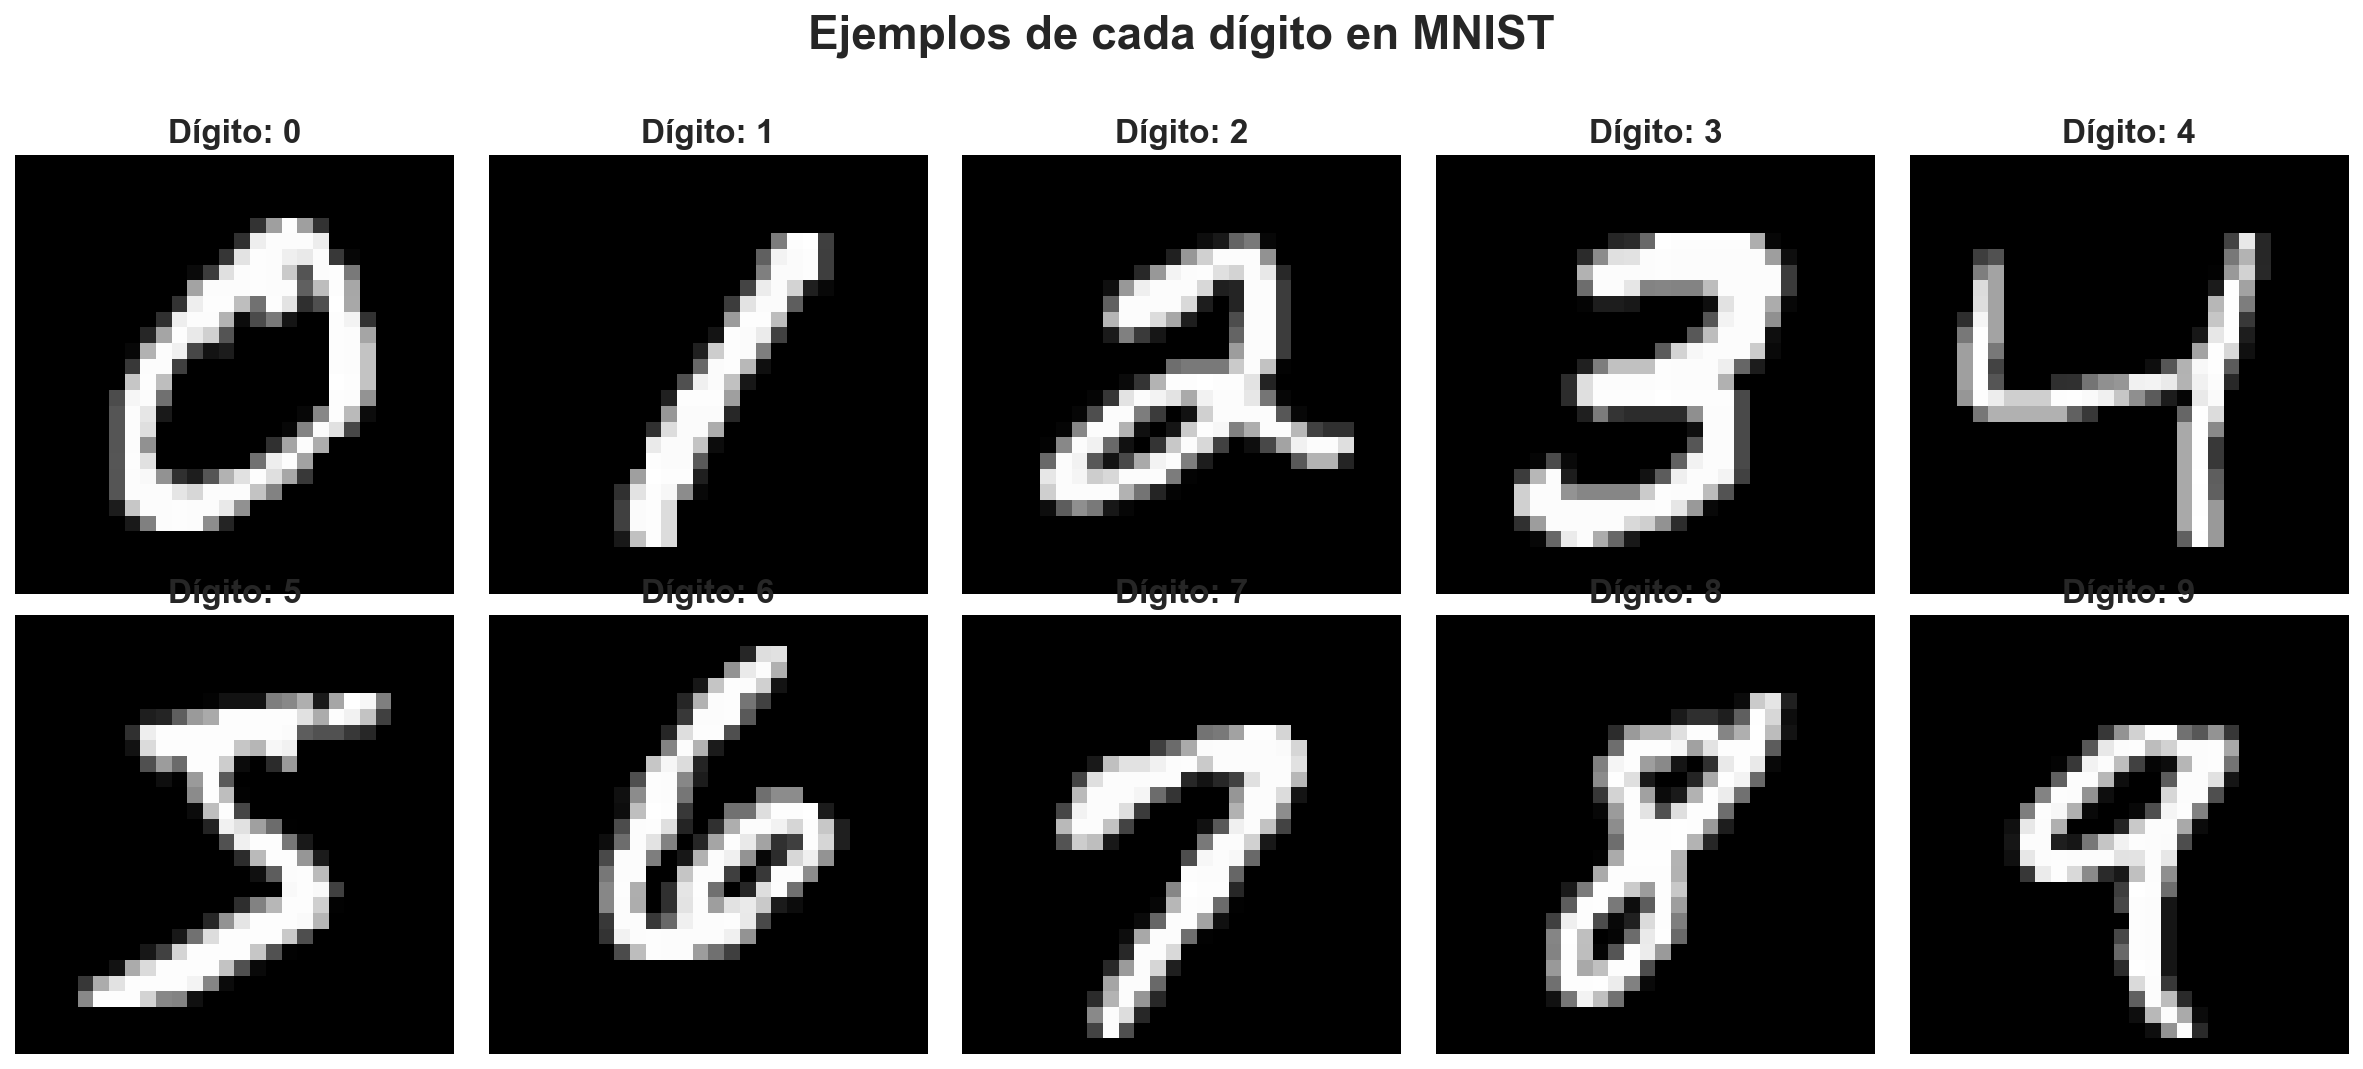
\includegraphics[width=\linewidth]{ejemplos_mnist.png}

    \small Ejemplos de digitos en MNIST
\end{center}
\end{columns}
\end{frame}

%========== SLIDE 3: EDA ==========
\begin{frame}{Exploracion del Dataset}
\begin{columns}
\column{0.5\textwidth}
\begin{center}
    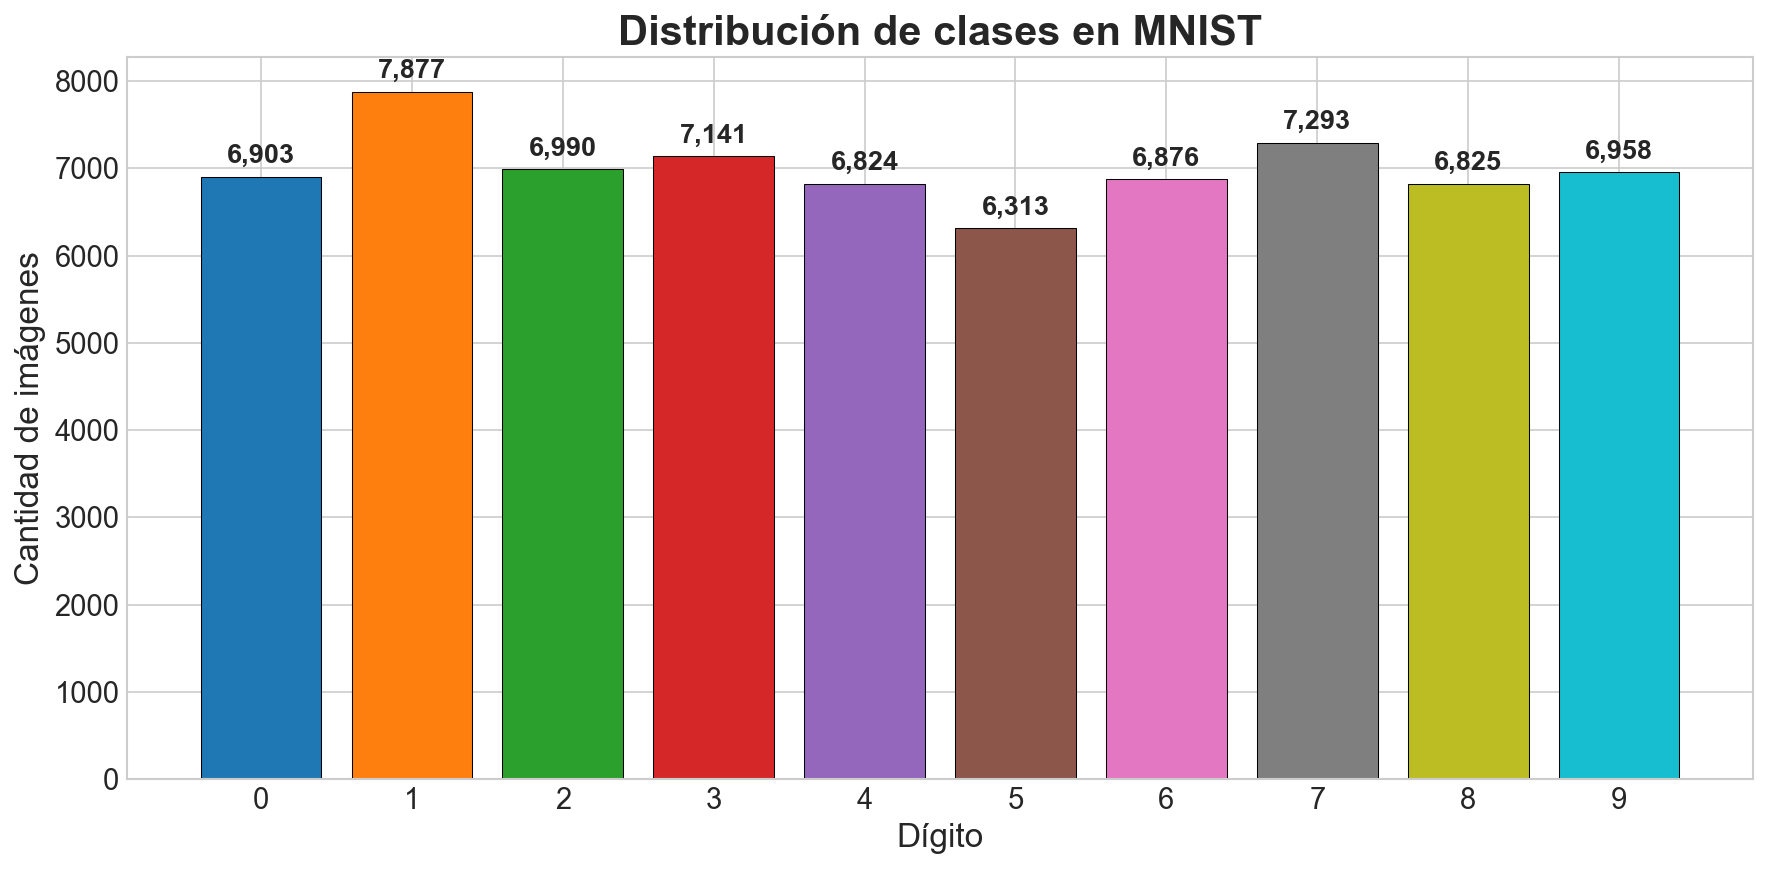
\includegraphics[width=\linewidth]{distribucion_clases.png}

    \small Distribucion de clases balanceada
\end{center}

\column{0.5\textwidth}
\begin{center}
    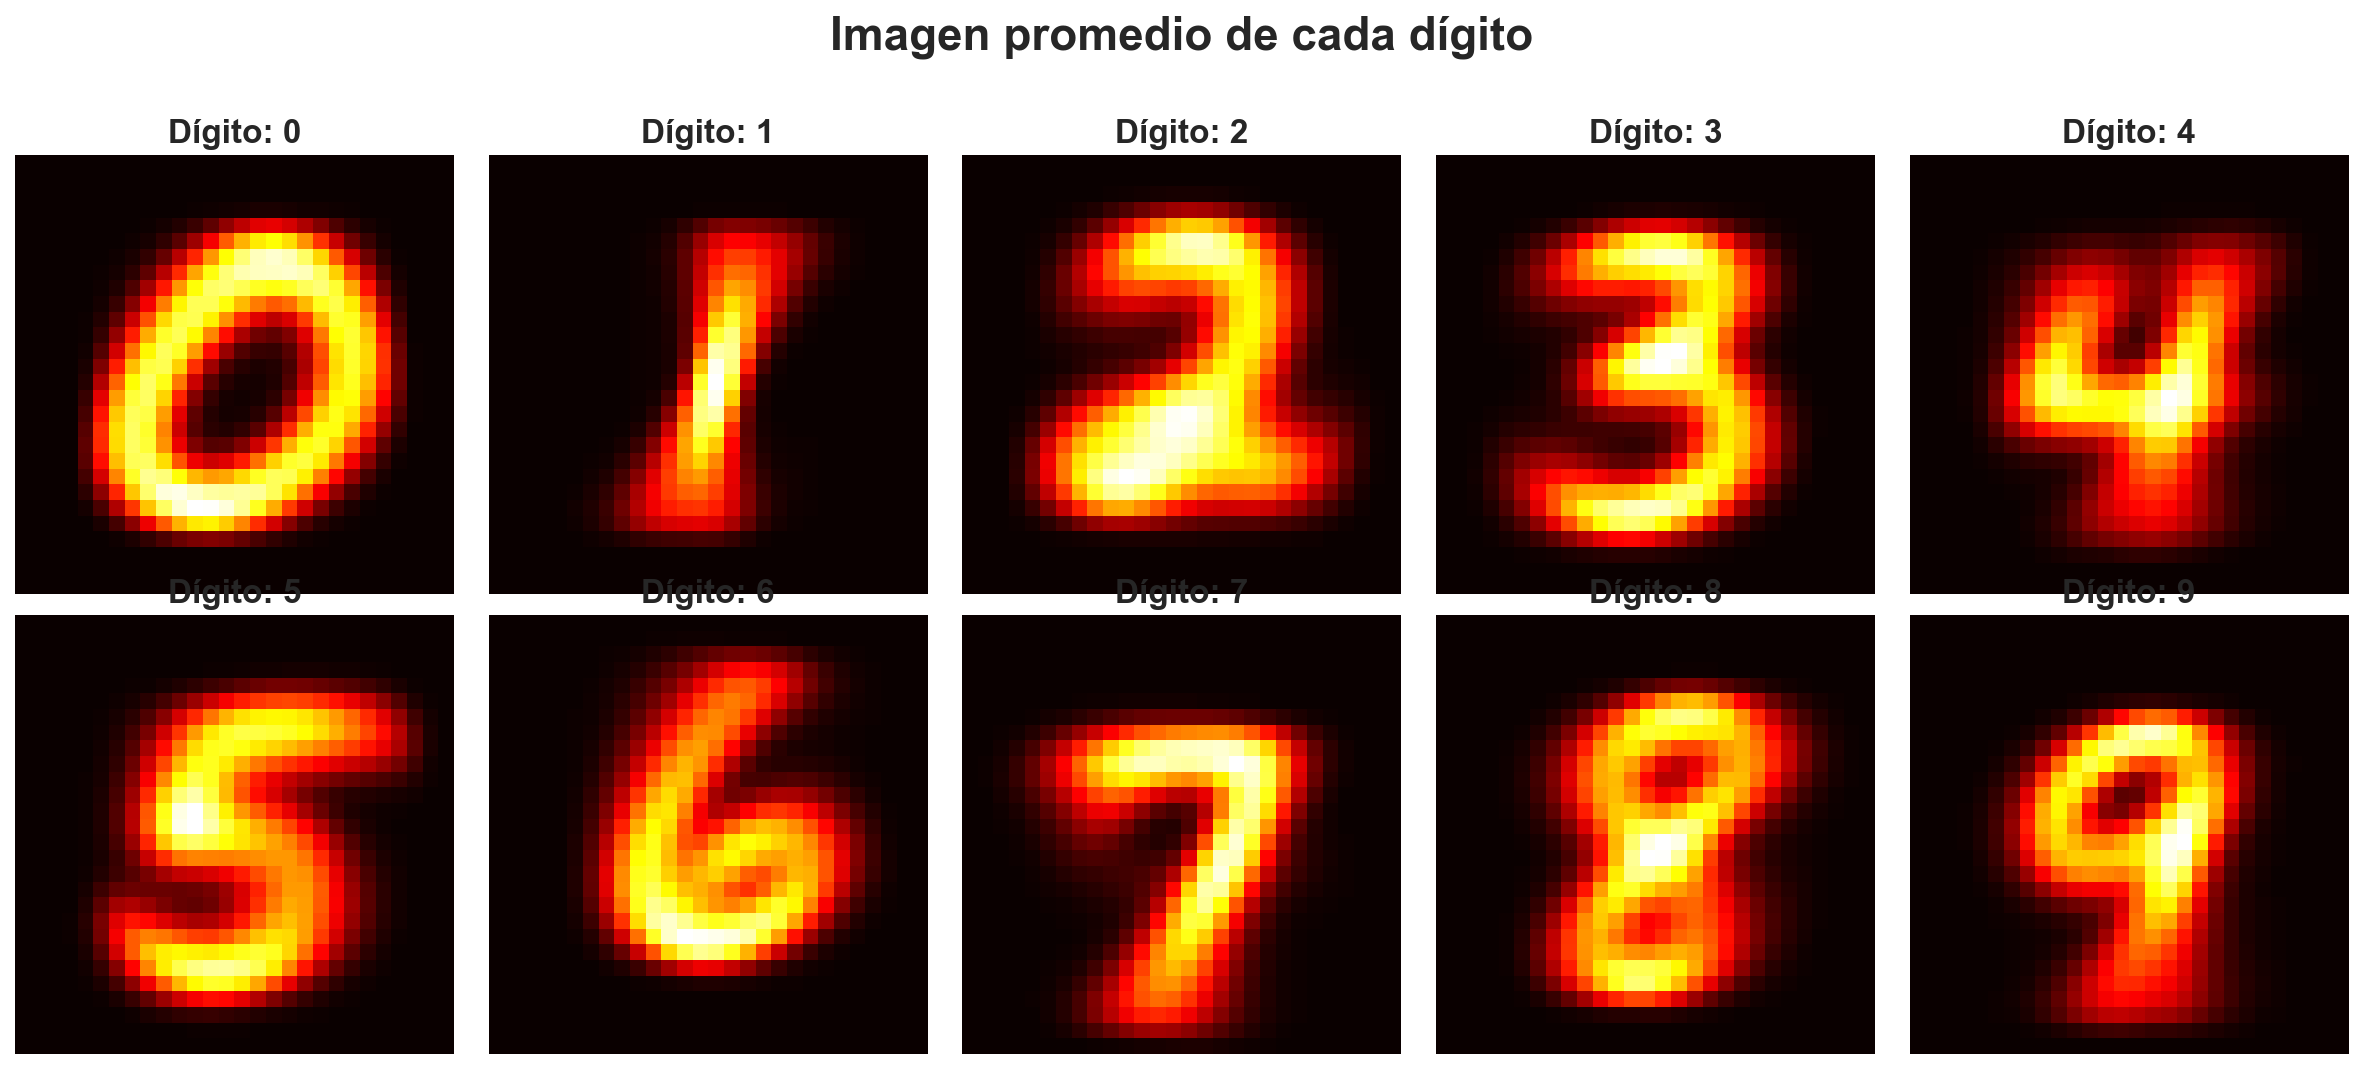
\includegraphics[width=\linewidth]{promedios_digitos.png}

    \small Imagen promedio por digito
\end{center}
\end{columns}

\vspace{0.3cm}
\begin{itemize}
    \item Las clases estan \textbf{balanceadas} ($\sim$6,000--7,000 por digito)
    \item Las imagenes promedio muestran los \textbf{patrones caracteristicos} de cada digito
\end{itemize}
\end{frame}

%========== SLIDE 4: MODELO ==========
\begin{frame}{Modelo: Red Neuronal MLP}
\begin{columns}
\column{0.5\textwidth}
\textbf{Arquitectura:}
\begin{center}
\begin{tabular}{ll}
\toprule
\textbf{Capa} & \textbf{Neuronas} \\
\midrule
Entrada & 784 (28$\times$28 px) \\
Oculta 1 & 256 (ReLU) \\
Oculta 2 & 128 (ReLU) \\
Oculta 3 & 64 (ReLU) \\
Salida & 10 (digitos 0--9) \\
\bottomrule
\end{tabular}
\end{center}

\vspace{0.3cm}
\textbf{Hiperparametros:}
\begin{itemize}
    \item Optimizador: Adam (lr=0.001)
    \item Batch size: 256
    \item Max epochs: 50
\end{itemize}

\column{0.5\textwidth}
\textbf{Data Augmentation:}
\begin{itemize}
    \item 30,000 imagenes extras generadas
    \item Desplazamientos aleatorios ($\pm$2px)
    \item Rotaciones aleatorias ($\pm$10\textdegree)
    \item Ruido gaussiano + escala de intensidad
    \item Total entrenamiento: 90,000 imagenes
\end{itemize}

\vspace{0.3cm}
\textbf{¿Por que augmentation?}
\begin{itemize}
    \item Mejorar robustez a variaciones reales
    \item Simular diferencias de escritura y posicion
\end{itemize}
\end{columns}
\end{frame}

%========== SLIDE 5: ENTRENAMIENTO ==========
\begin{frame}{Entrenamiento}
\begin{columns}
\column{0.55\textwidth}
\begin{center}
    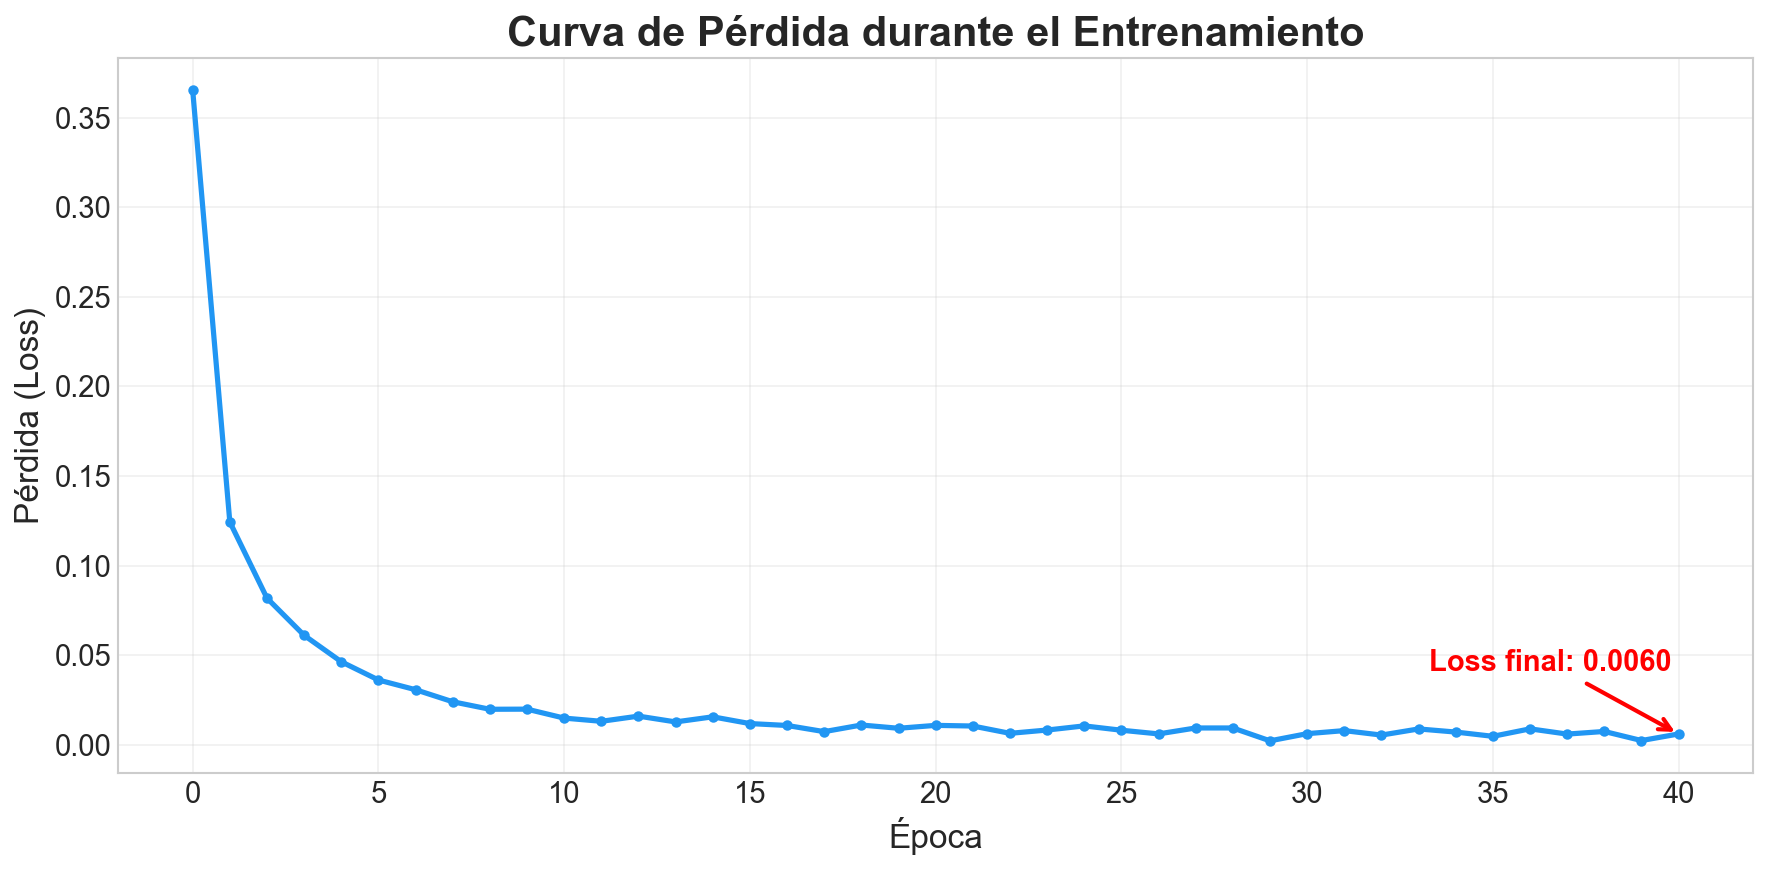
\includegraphics[width=\linewidth]{curva_perdida.png}

    \small Curva de perdida durante el entrenamiento
\end{center}

\column{0.4\textwidth}
\begin{itemize}
    \item La perdida \textbf{disminuye} consistentemente
    \item El modelo \textbf{converge} en $\sim$38 epocas
    \item No se observa sobreajuste significativo
\end{itemize}

\vspace{0.3cm}
\textbf{Resultados en MNIST test:}
\begin{itemize}
    \item \textbf{Accuracy: 98.43\%}
    \item Solo 157 errores de 10,000
\end{itemize}
\end{columns}
\end{frame}

%========== SLIDE 6: EVALUACION MNIST ==========
\begin{frame}{Evaluacion en MNIST}
\begin{columns}
\column{0.5\textwidth}
\begin{center}
    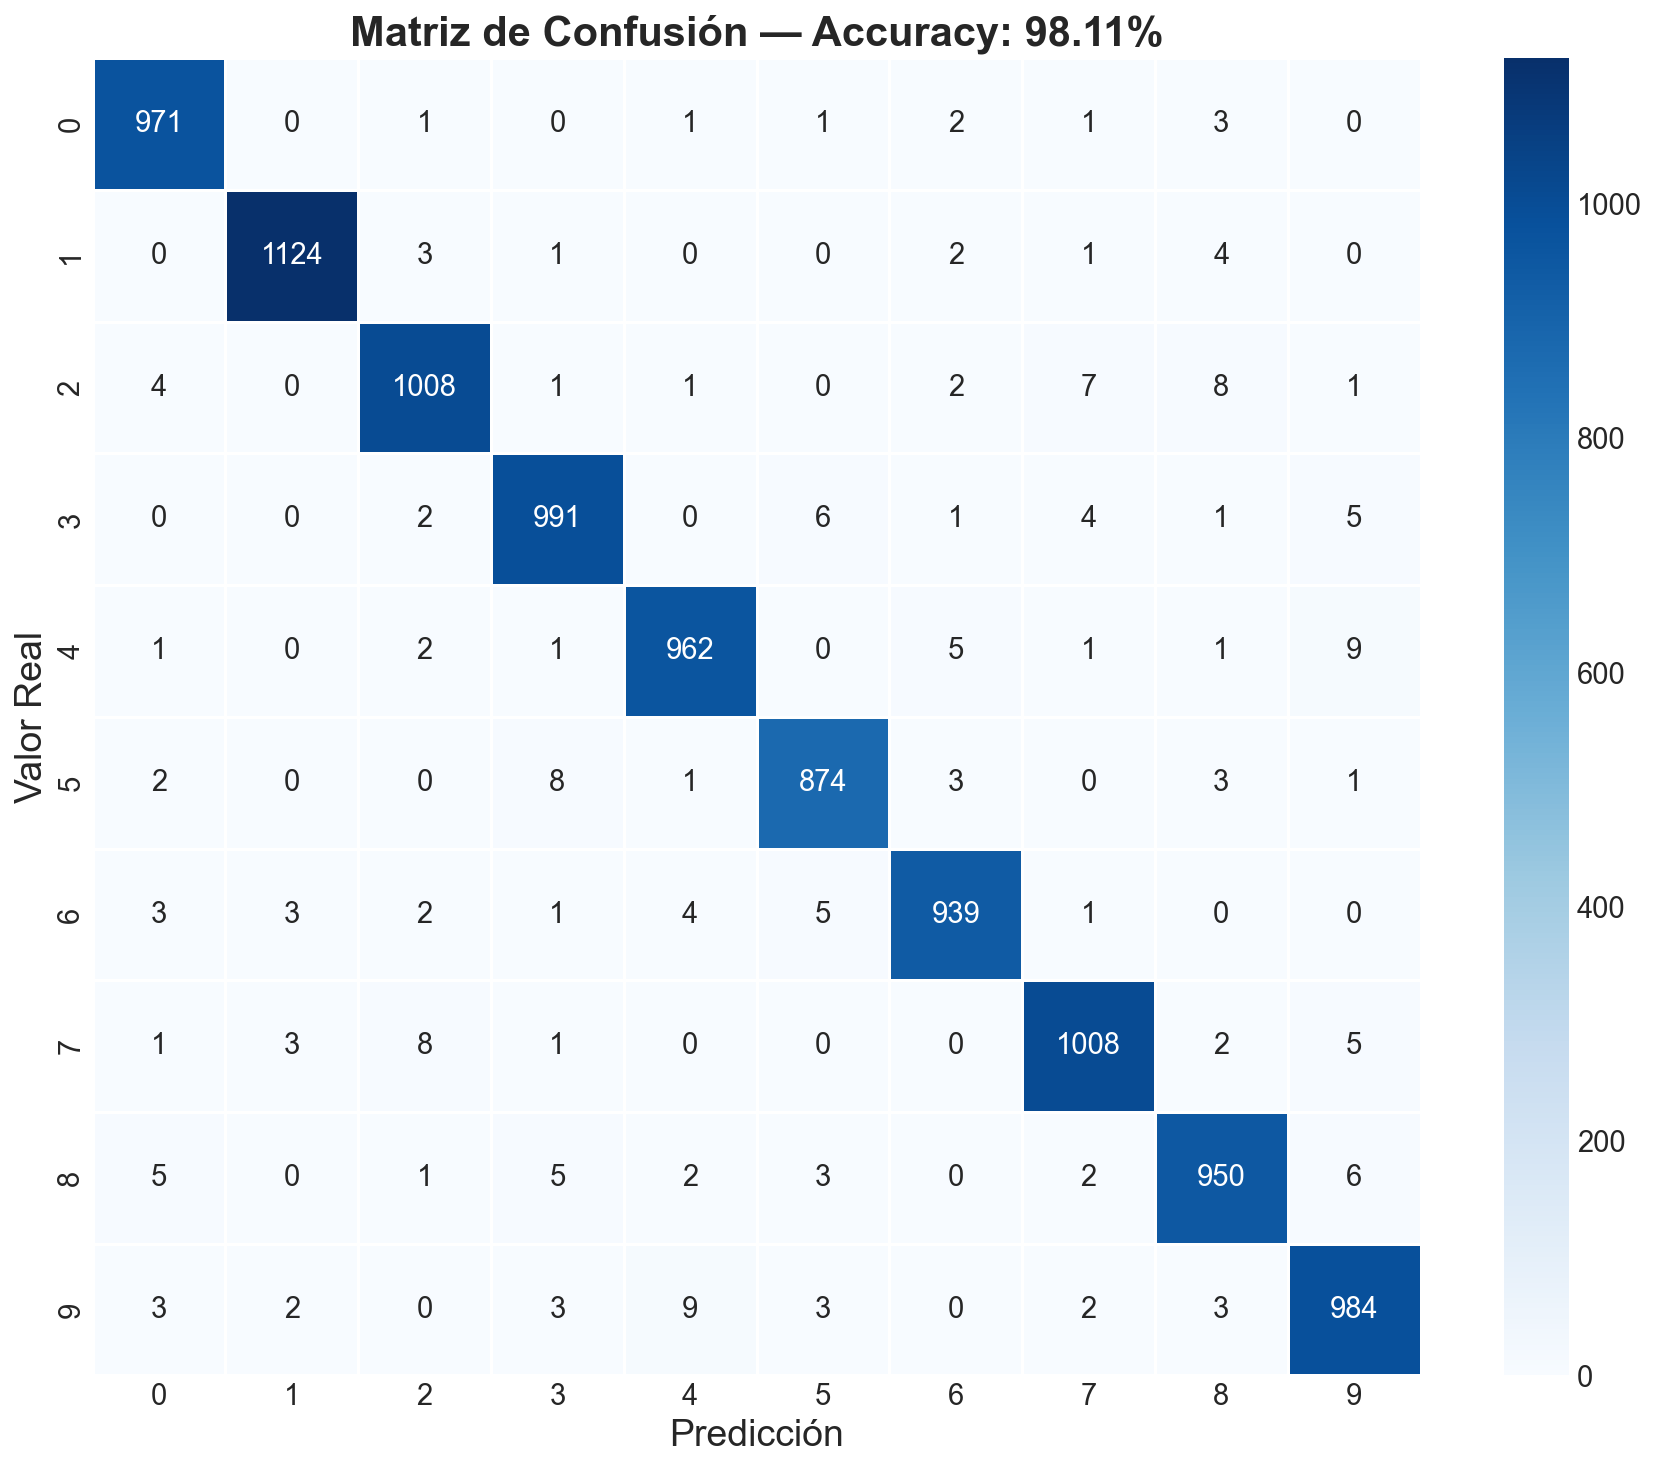
\includegraphics[width=\linewidth]{matriz_confusion.png}
\end{center}

\column{0.5\textwidth}
\begin{center}
    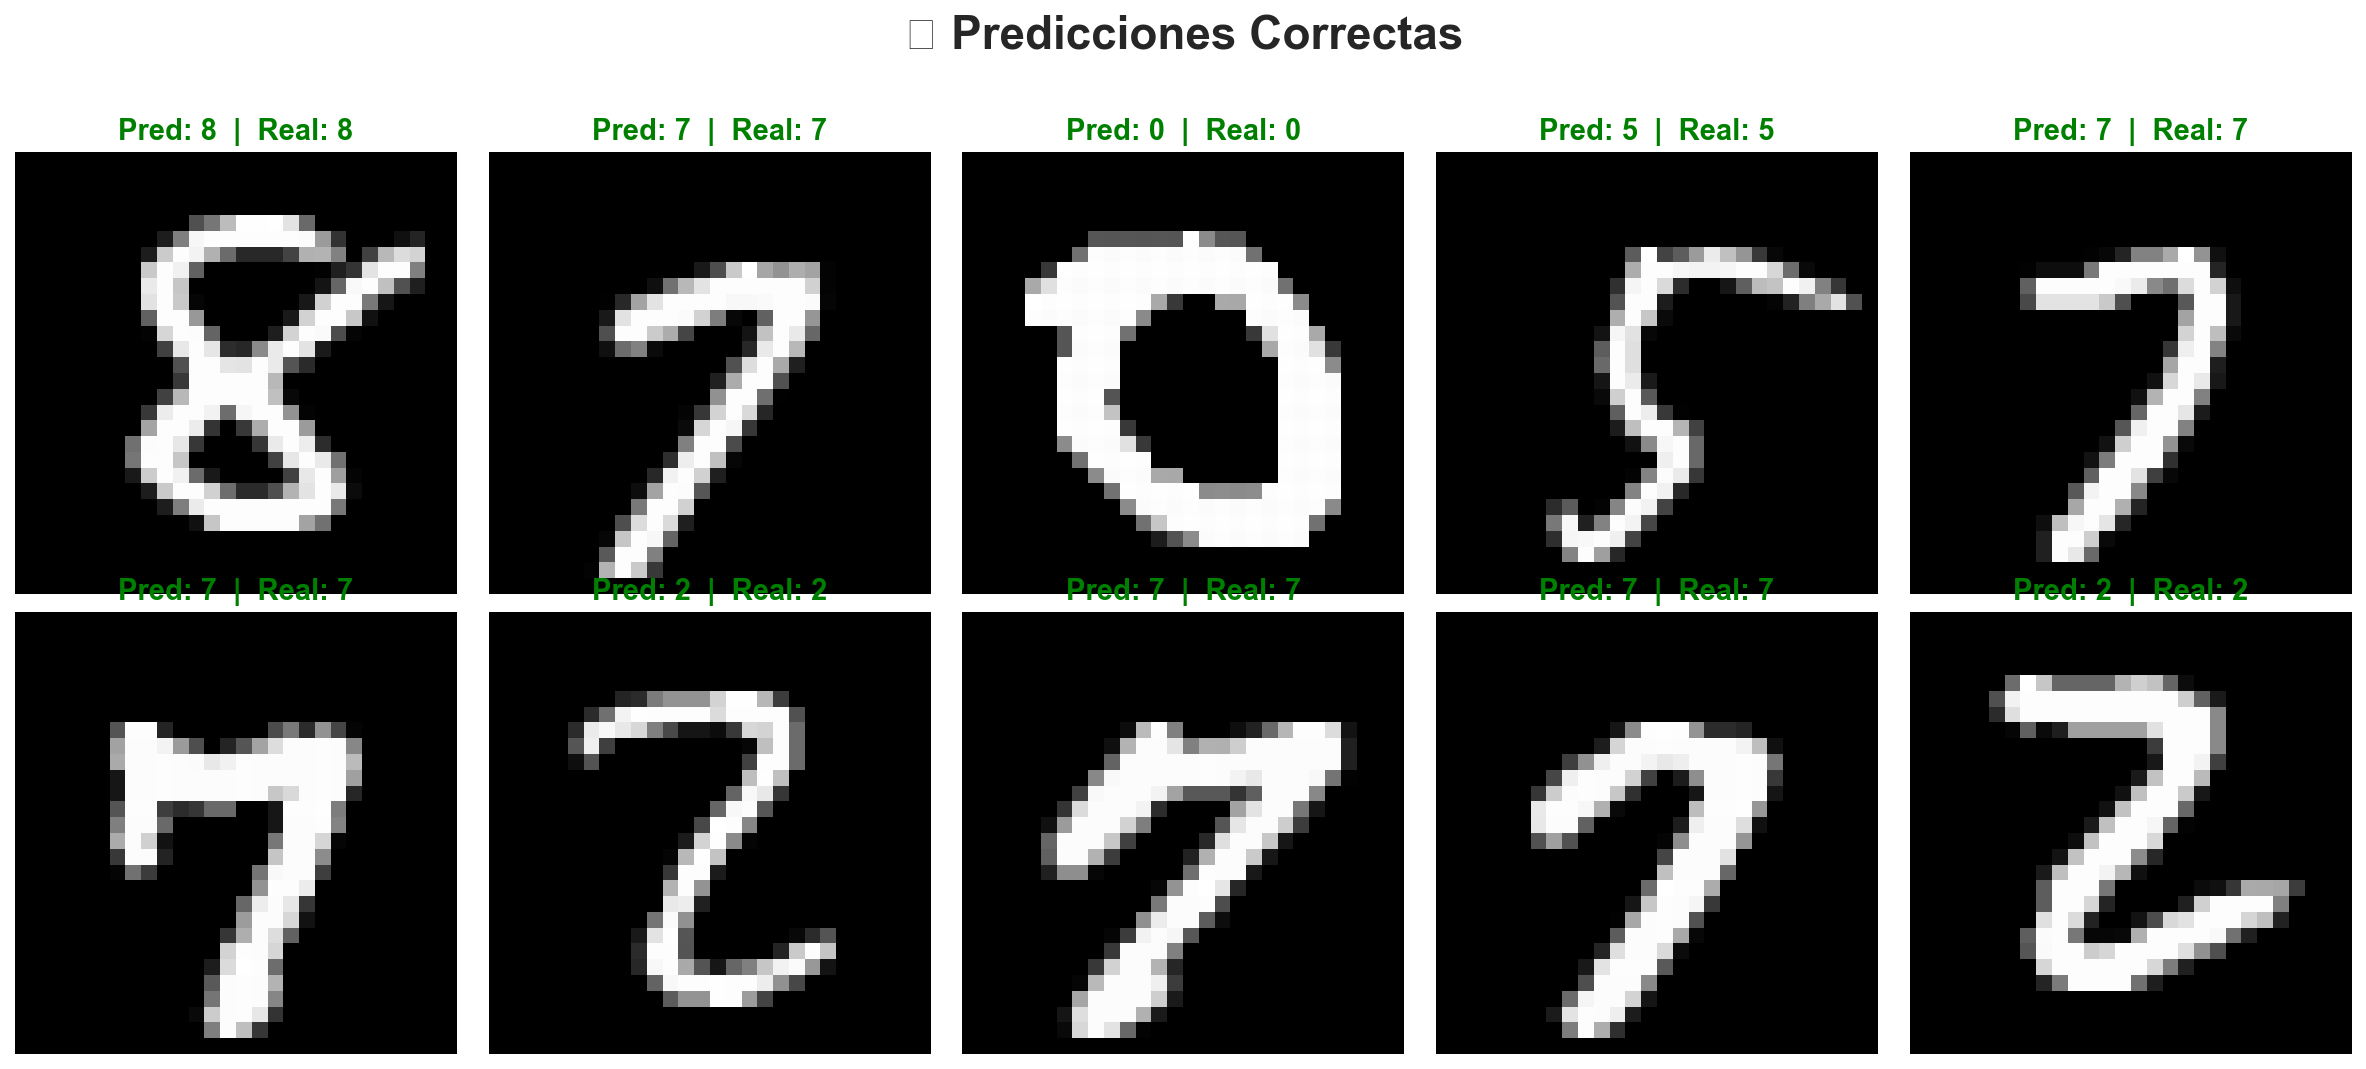
\includegraphics[width=0.95\linewidth]{predicciones_correctas.png}

    \small Ejemplos de predicciones correctas
\end{center}

\vspace{0.2cm}
\textbf{Observaciones:}
\begin{itemize}
    \item Diagonal dominante $\rightarrow$ pocas confusiones
    \item Pares confundidos: (3,5), (4,9), (7,1)
\end{itemize}
\end{columns}
\end{frame}

%========== SLIDE 7: PREPROCESAMIENTO ==========
\begin{frame}{Preprocesamiento de Imagenes Propias}
\begin{columns}
\column{0.5\textwidth}
\textbf{Pipeline adaptativo por tamaño:}

\vspace{0.2cm}
\textbf{Fotos pequeñas} (<300px, recortes):
\begin{itemize}
    \item Umbral adaptativo
    \item Conservar valores de gris
    \item Dilatacion morfologica
\end{itemize}

\vspace{0.2cm}
\textbf{Fotos grandes} (>300px, pagina):
\begin{itemize}
    \item Filtro mediana fuerte
    \item Binarizacion + componentes conectados
    \item Erosion (>900px) para aislar digito
    \item Dilatacion para restaurar trazos
\end{itemize}

\column{0.5\textwidth}
\begin{center}
    \includegraphics[width=\linewidth]{antes_despues.png}

    \small Antes y despues del preprocesamiento
\end{center}
\end{columns}

\vspace{0.2cm}
\begin{alertblock}{Importante}
Las imagenes propias \textbf{NO} se usaron para entrenar --- solo para \textbf{probar} el modelo.
\end{alertblock}
\end{frame}

%========== SLIDE 8: RESULTADOS PROPIAS ==========
\begin{frame}{Resultados con Imagenes Propias}
\begin{columns}
\column{0.5\textwidth}
\begin{center}
    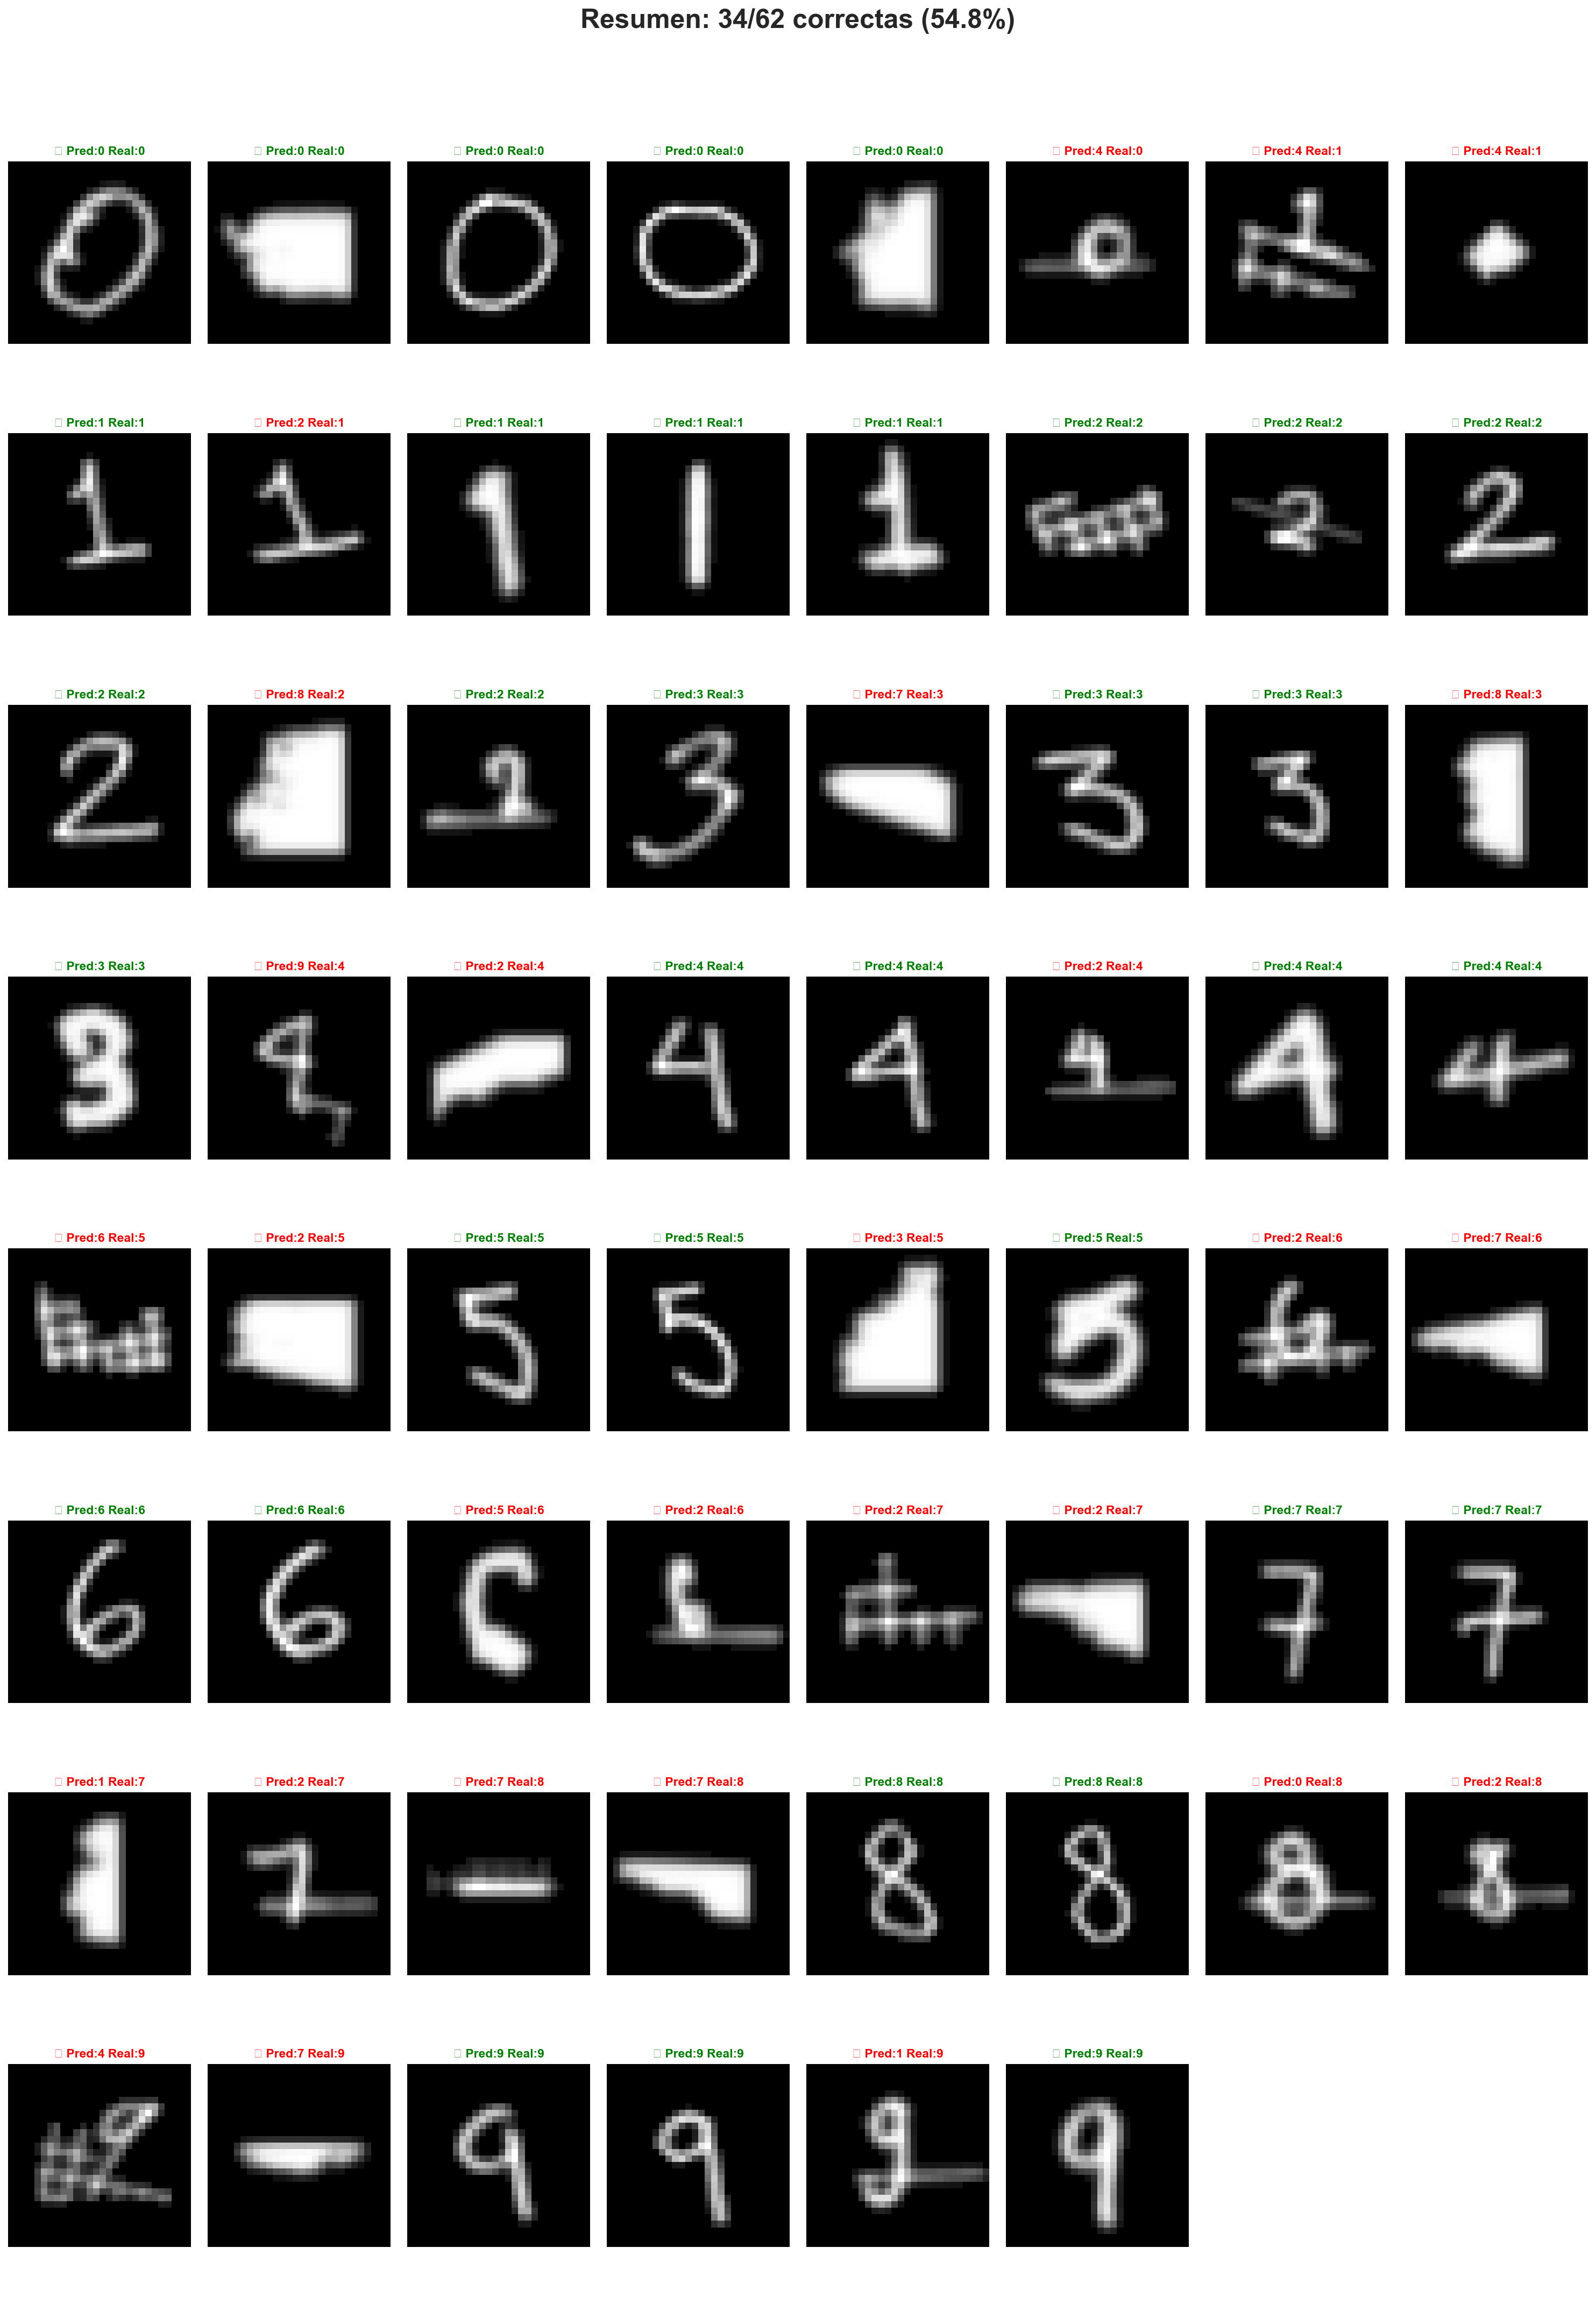
\includegraphics[width=\linewidth]{resumen_todas_predicciones.png}

    \small Resumen de todas las predicciones
\end{center}

\column{0.5\textwidth}
\begin{center}
    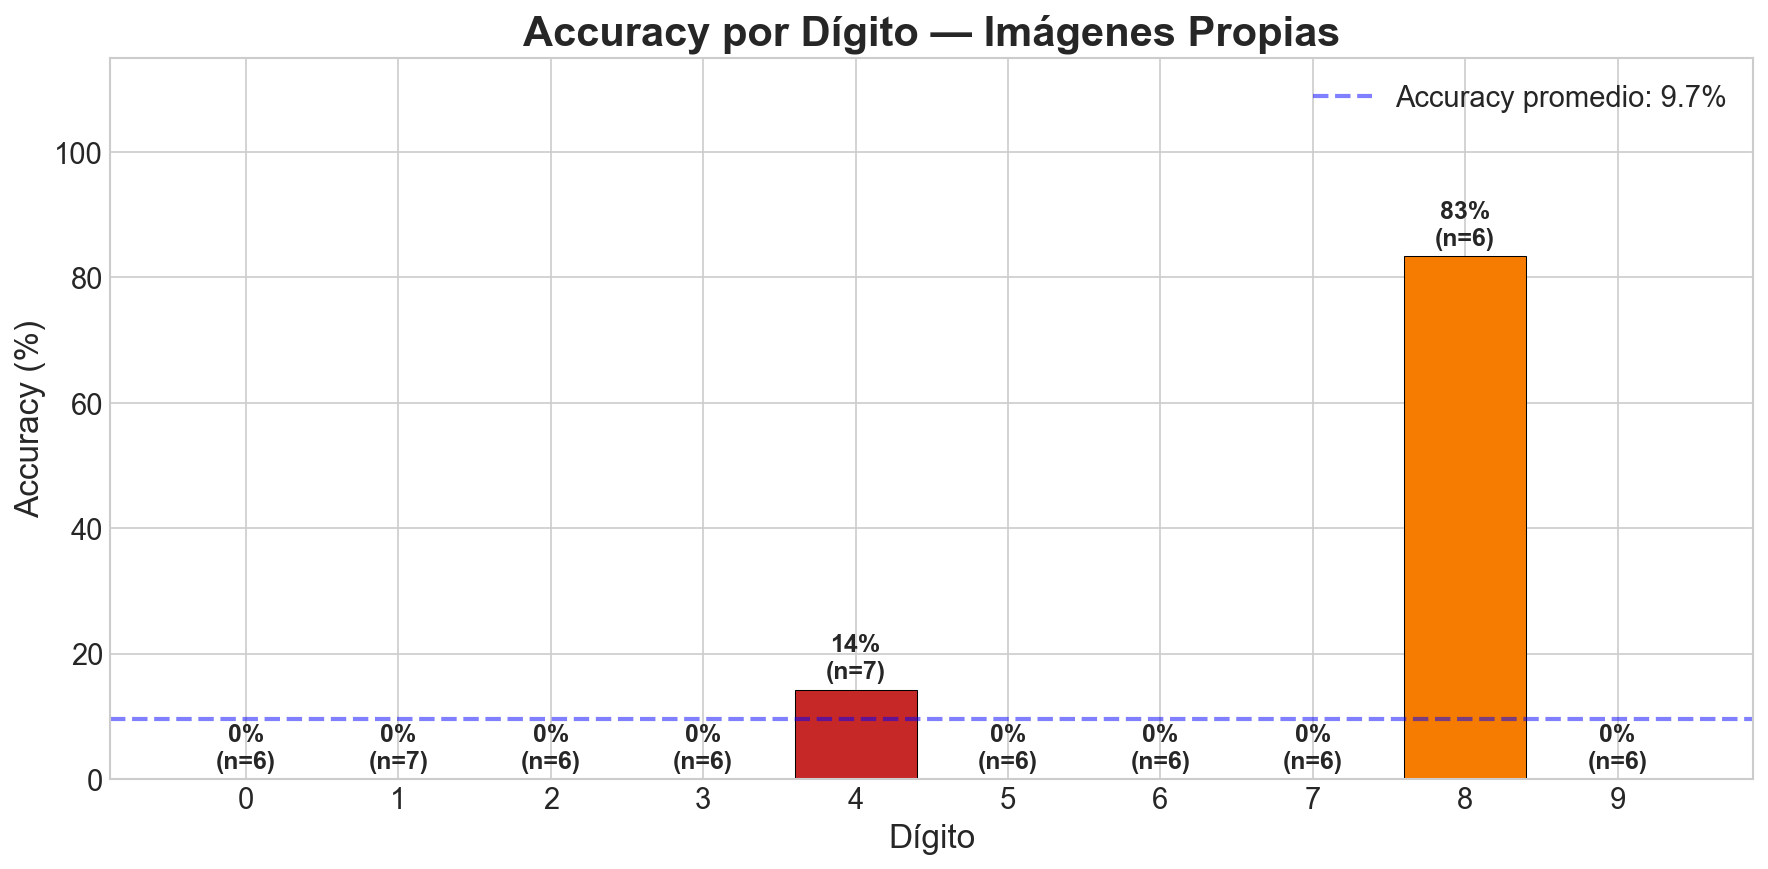
\includegraphics[width=\linewidth]{accuracy_por_digito.png}

    \small Accuracy por digito
\end{center}
\end{columns}

\vspace{0.2cm}
\begin{center}
\begin{tabular}{lcc}
\toprule
\textbf{Conjunto} & \textbf{Accuracy} & \textbf{Imagenes} \\
\midrule
MNIST test & 98.43\% & 10,000 \\
Imagenes propias (total) & $\sim$53\% & 62 \\
\quad Recortes pequeños (.jpeg) & $\sim$95\% & 20 \\
\quad Fotos de pagina (.jpg) & $\sim$33\% & 42 \\
\bottomrule
\end{tabular}
\end{center}
\end{frame}

%========== SLIDE 9: EJEMPLOS CORRECTOS ==========
\begin{frame}{Predicciones Correctas}
\begin{columns}
\column{0.5\textwidth}
\begin{center}
    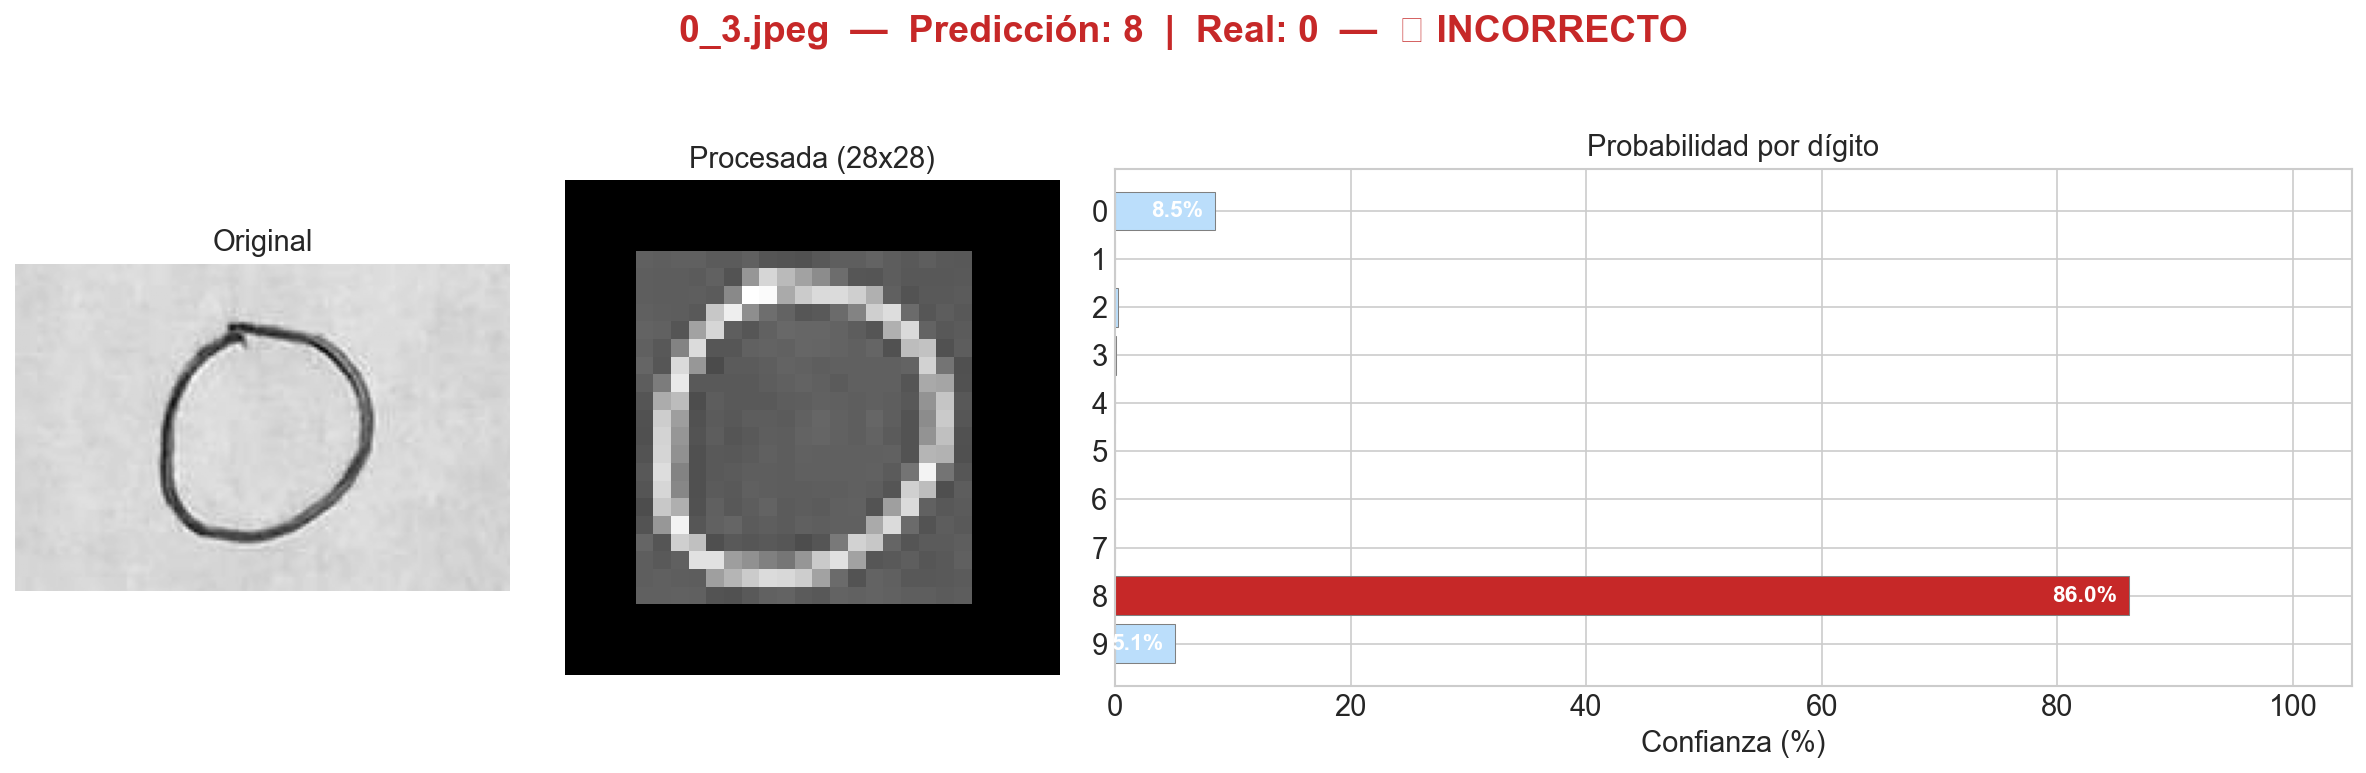
\includegraphics[width=\linewidth]{prediccion_0_3.png}

    \vspace{0.1cm}
    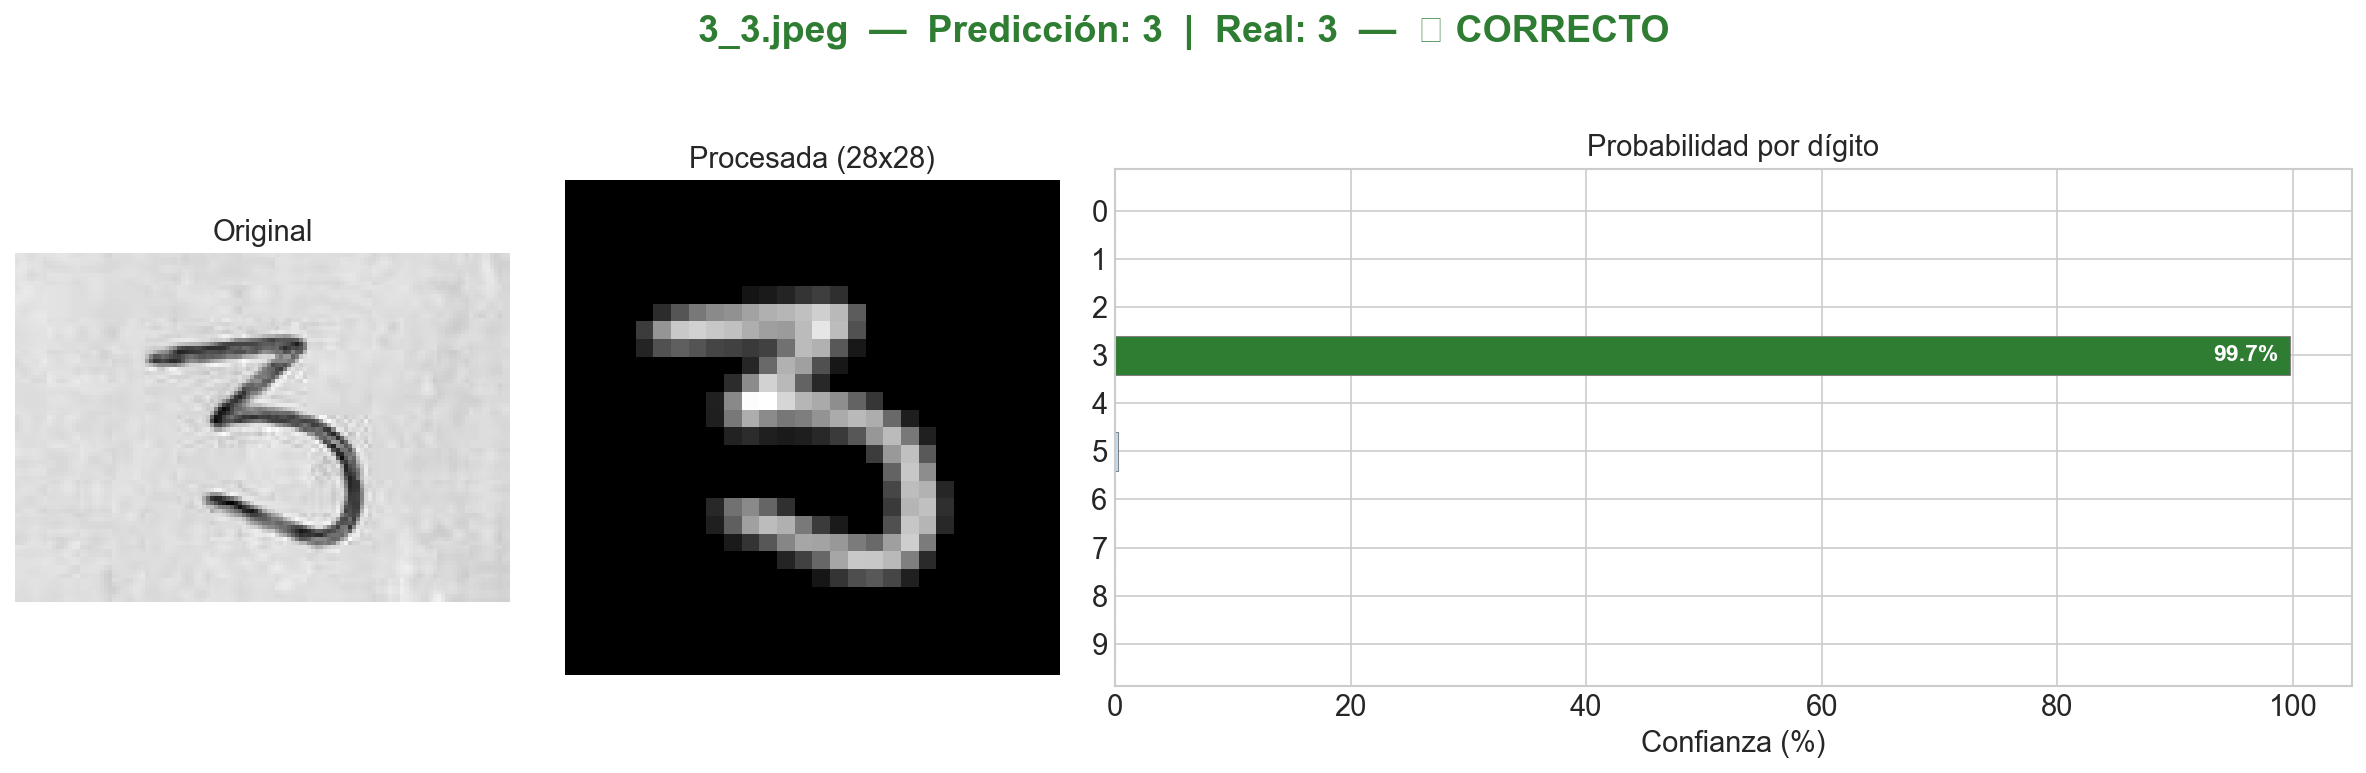
\includegraphics[width=\linewidth]{prediccion_3_3.png}
\end{center}

\column{0.5\textwidth}
\begin{center}
    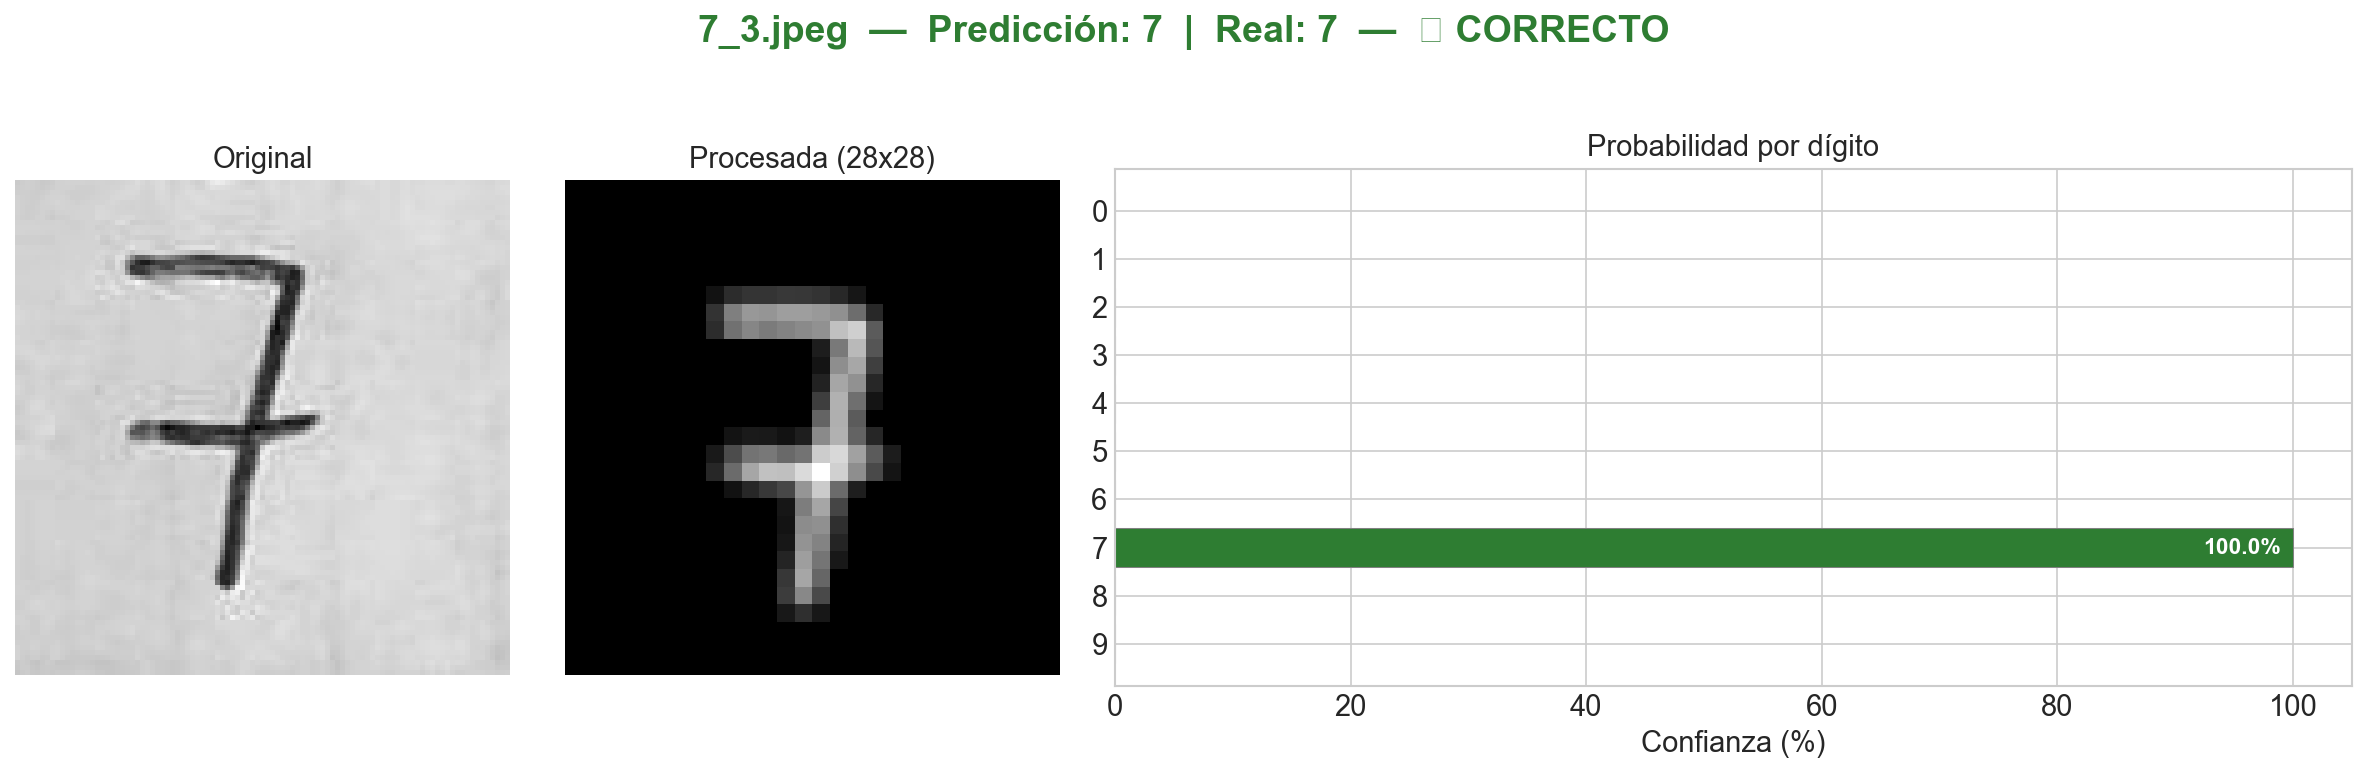
\includegraphics[width=\linewidth]{prediccion_7_3.png}

    \vspace{0.1cm}
    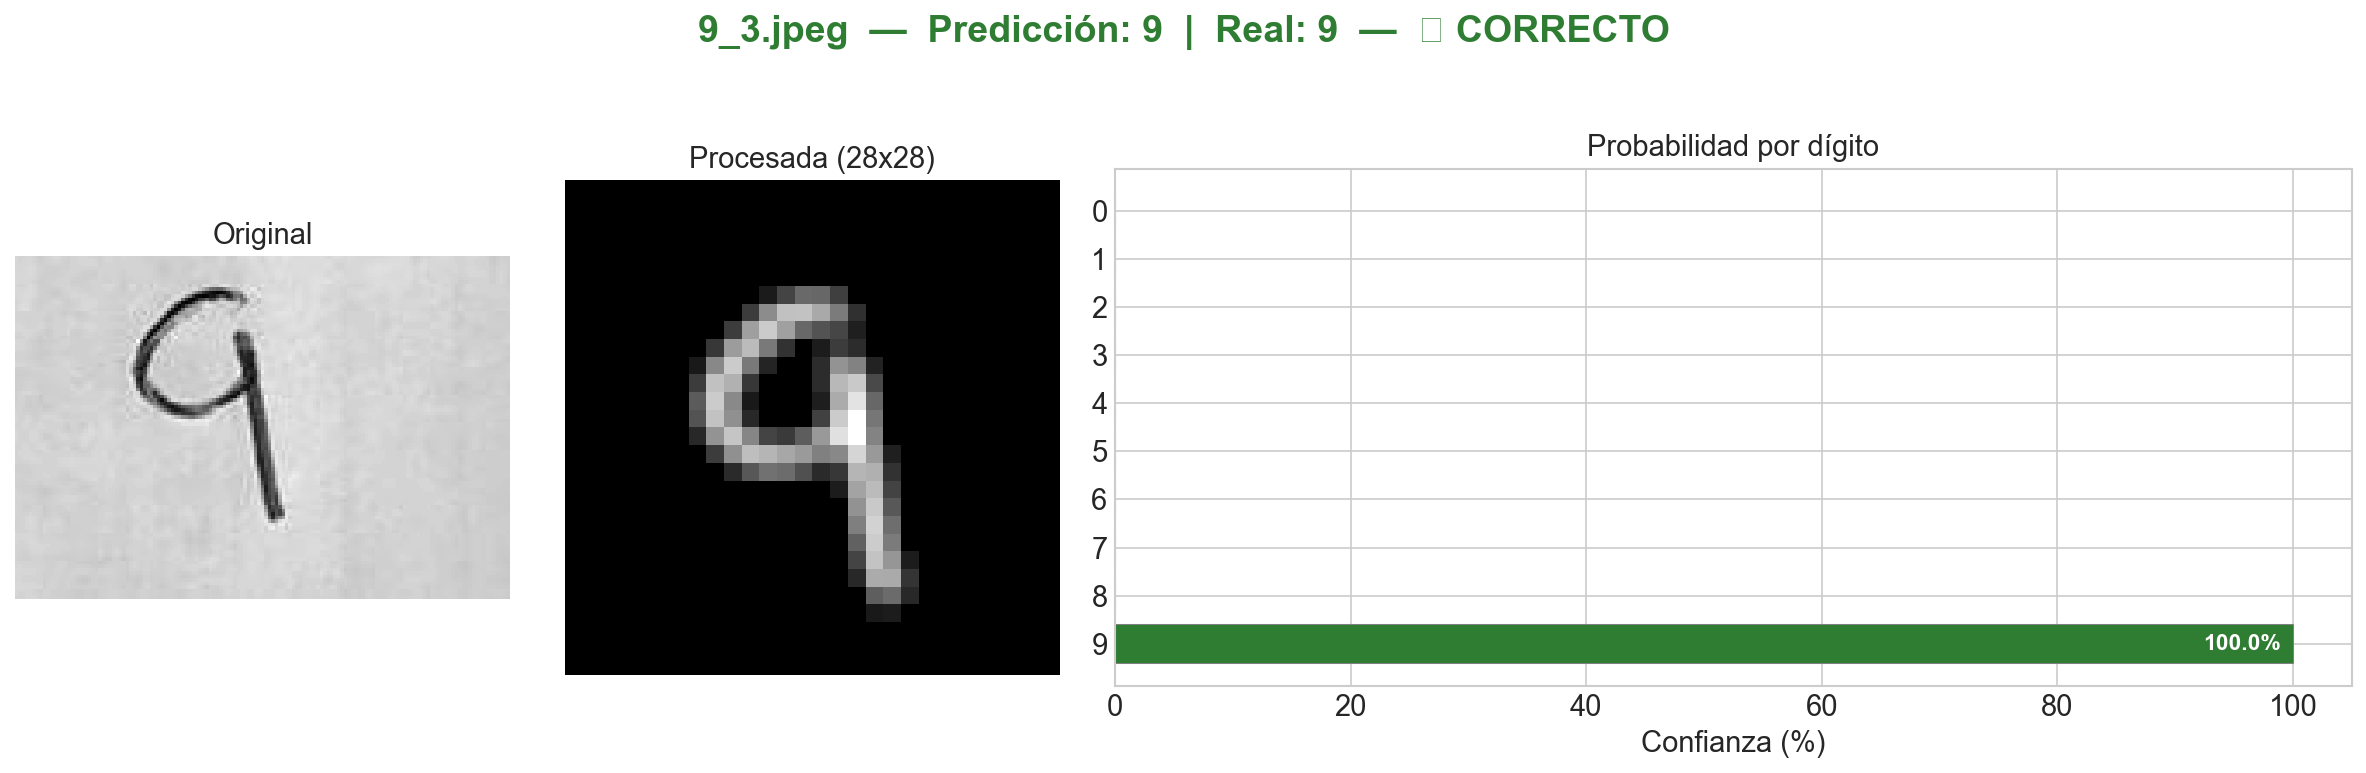
\includegraphics[width=\linewidth]{prediccion_9_3.png}
\end{center}
\end{columns}

\vspace{0.2cm}
\begin{center}
\small Imagenes bien recortadas y con trazo limpio $\rightarrow$ alta confianza (>95\%)
\end{center}
\end{frame}

%========== SLIDE 10: EJEMPLOS INCORRECTOS ==========
\begin{frame}{Predicciones Incorrectas --- ¿Por que falla?}
\begin{columns}
\column{0.5\textwidth}
\begin{center}
    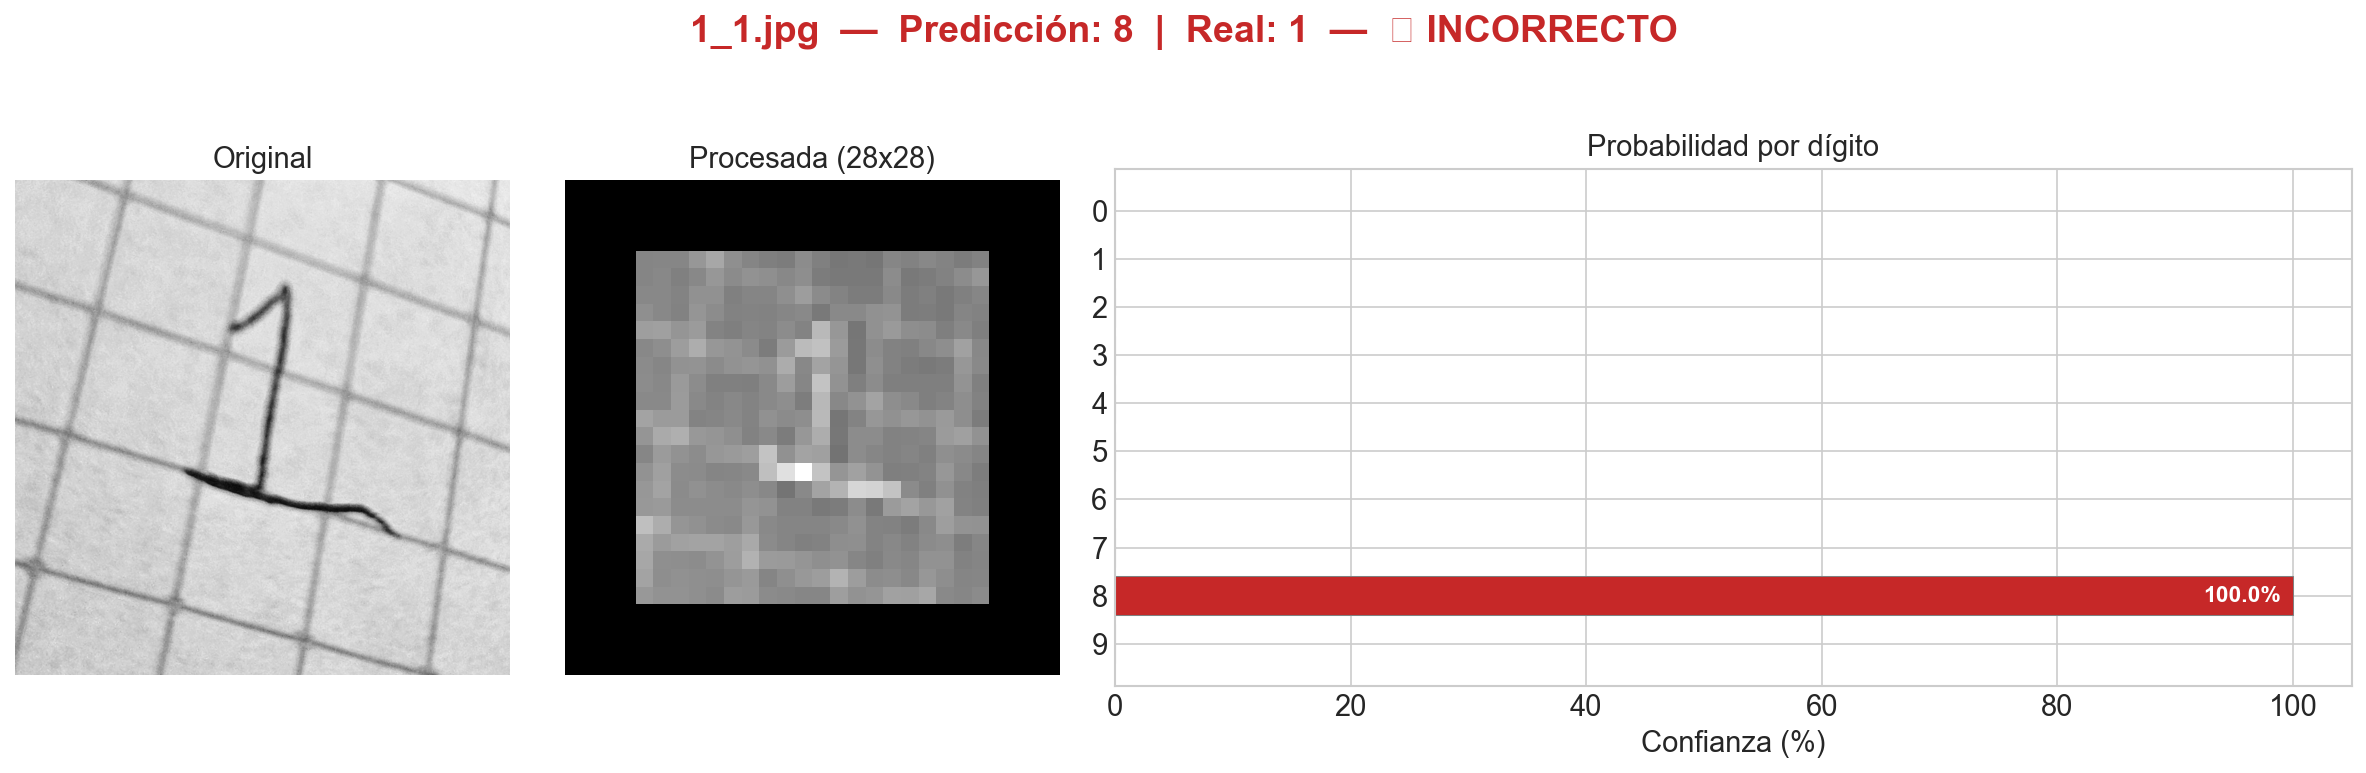
\includegraphics[width=\linewidth]{prediccion_1_1.png}

    \vspace{0.1cm}
    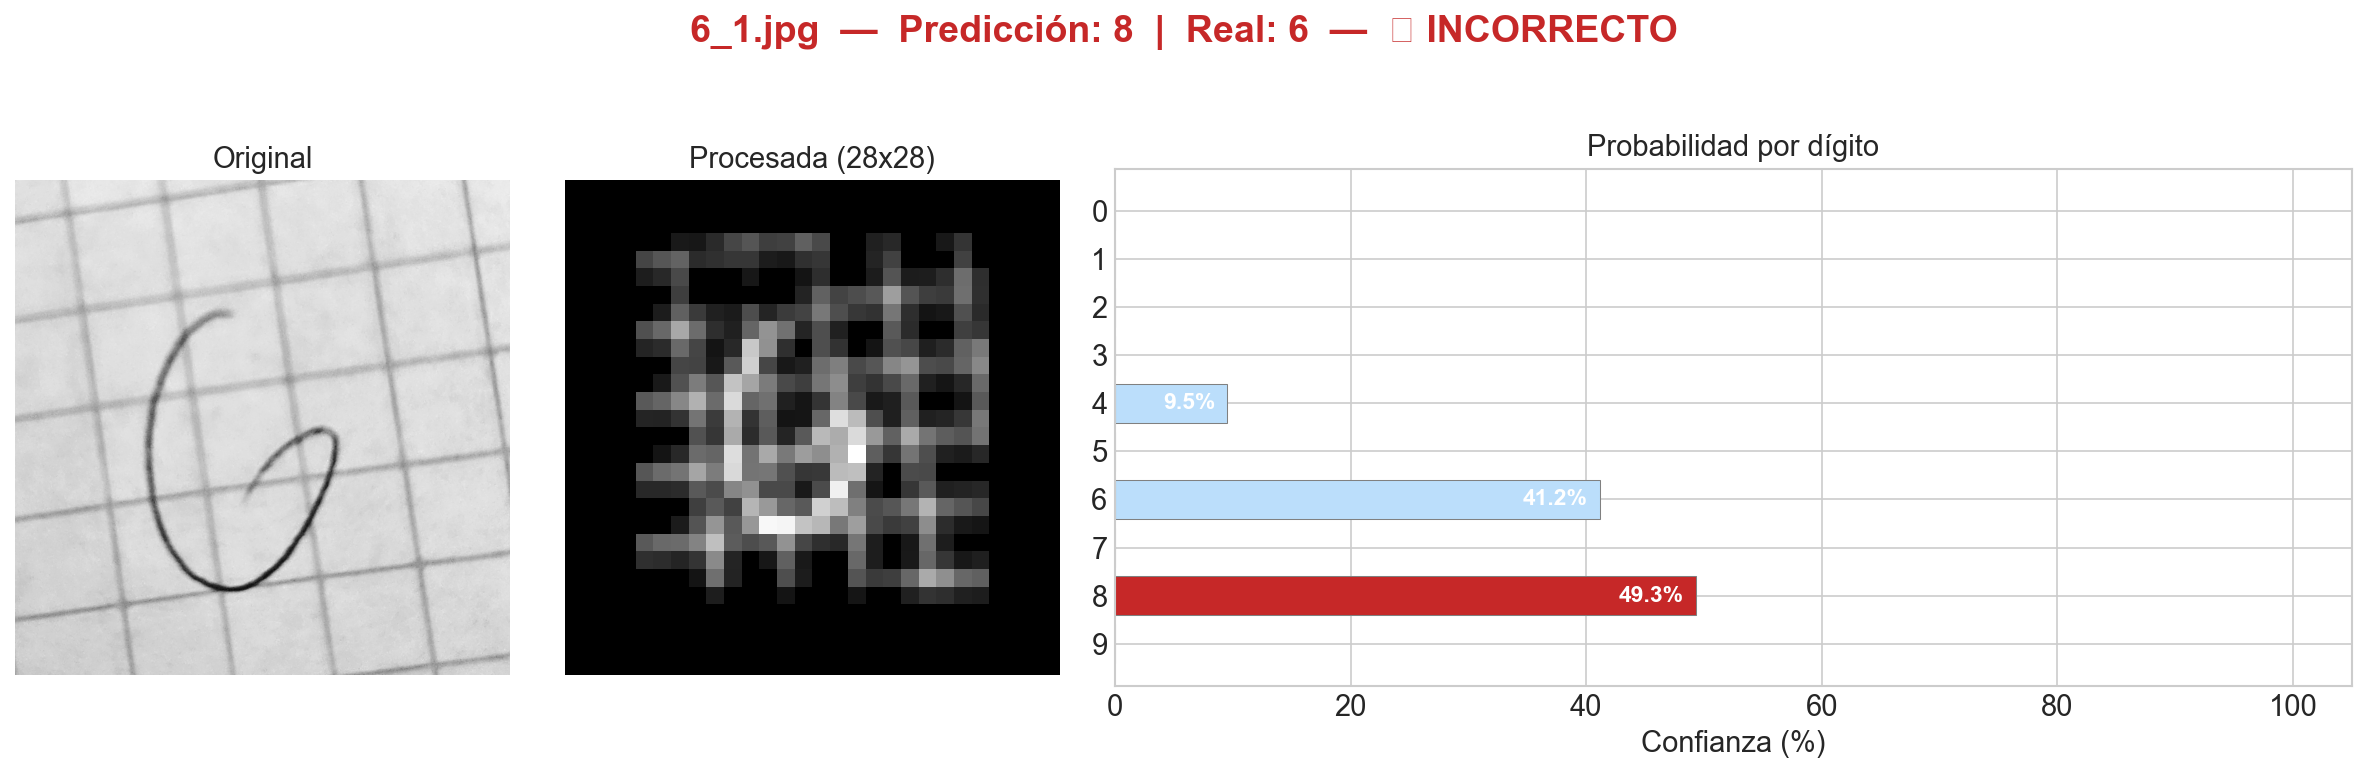
\includegraphics[width=\linewidth]{prediccion_6_1.png}
\end{center}

\column{0.5\textwidth}
\begin{center}
    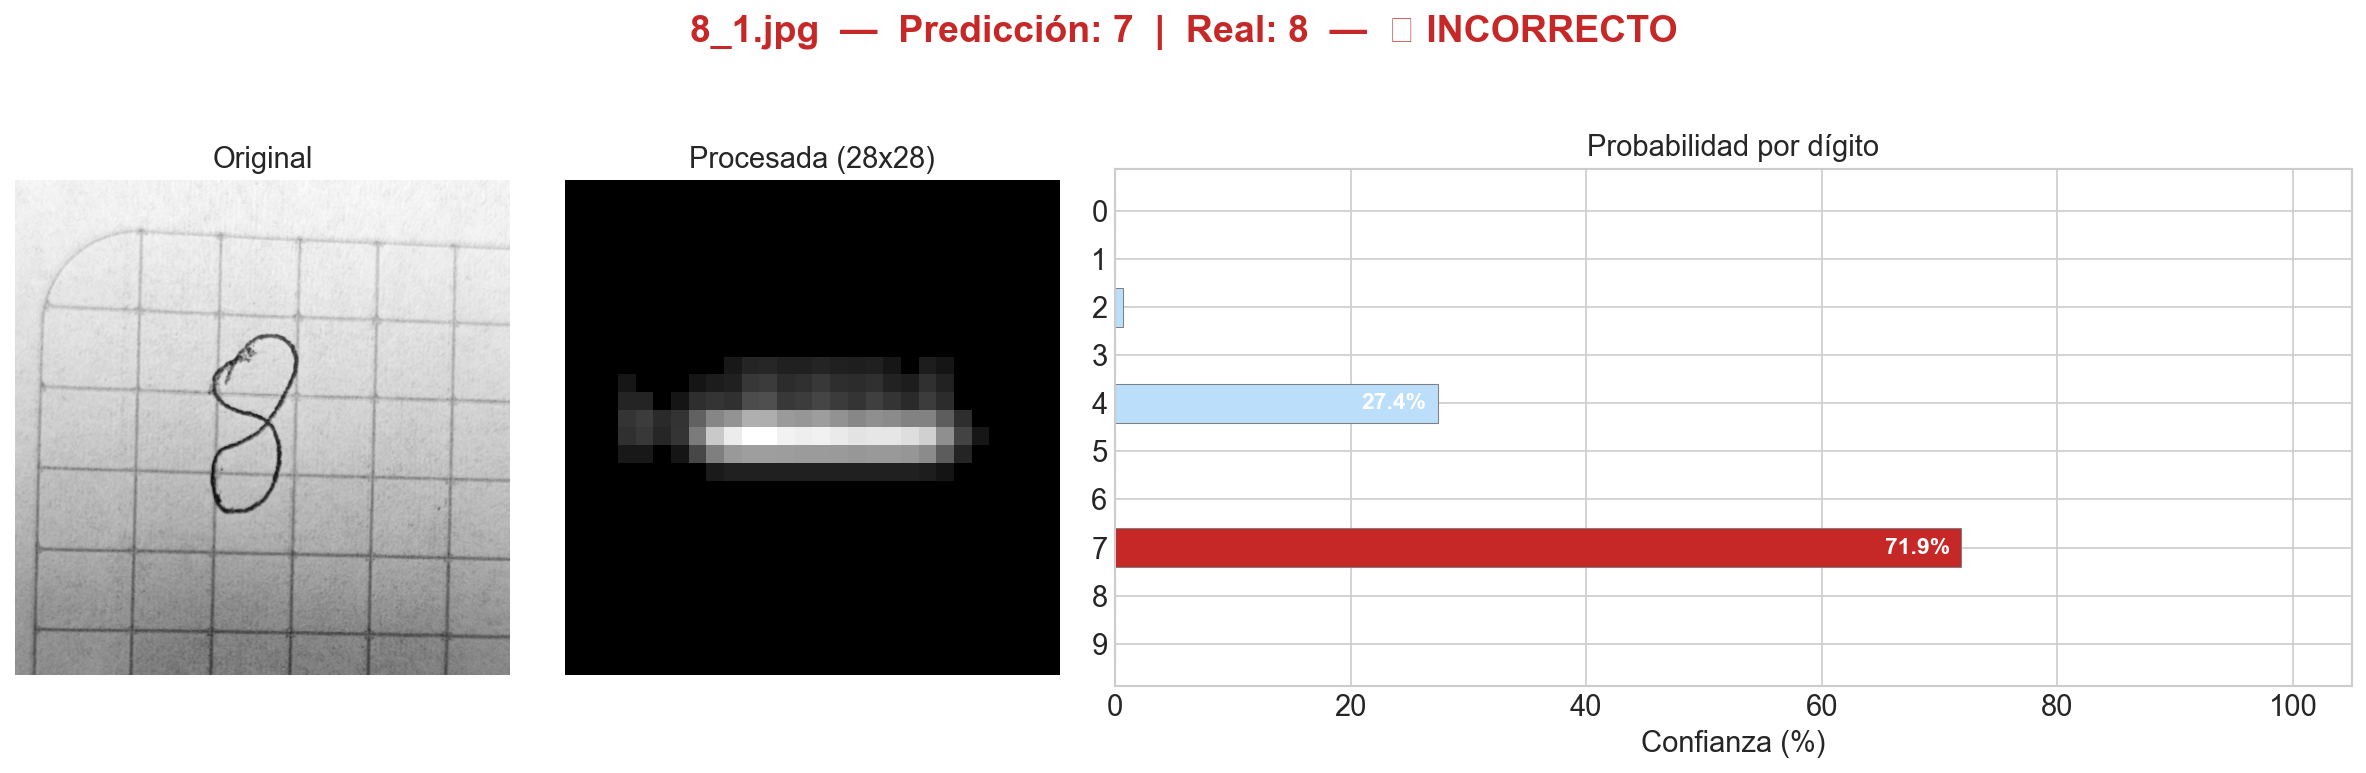
\includegraphics[width=\linewidth]{prediccion_8_1.png}

    \vspace{0.1cm}
    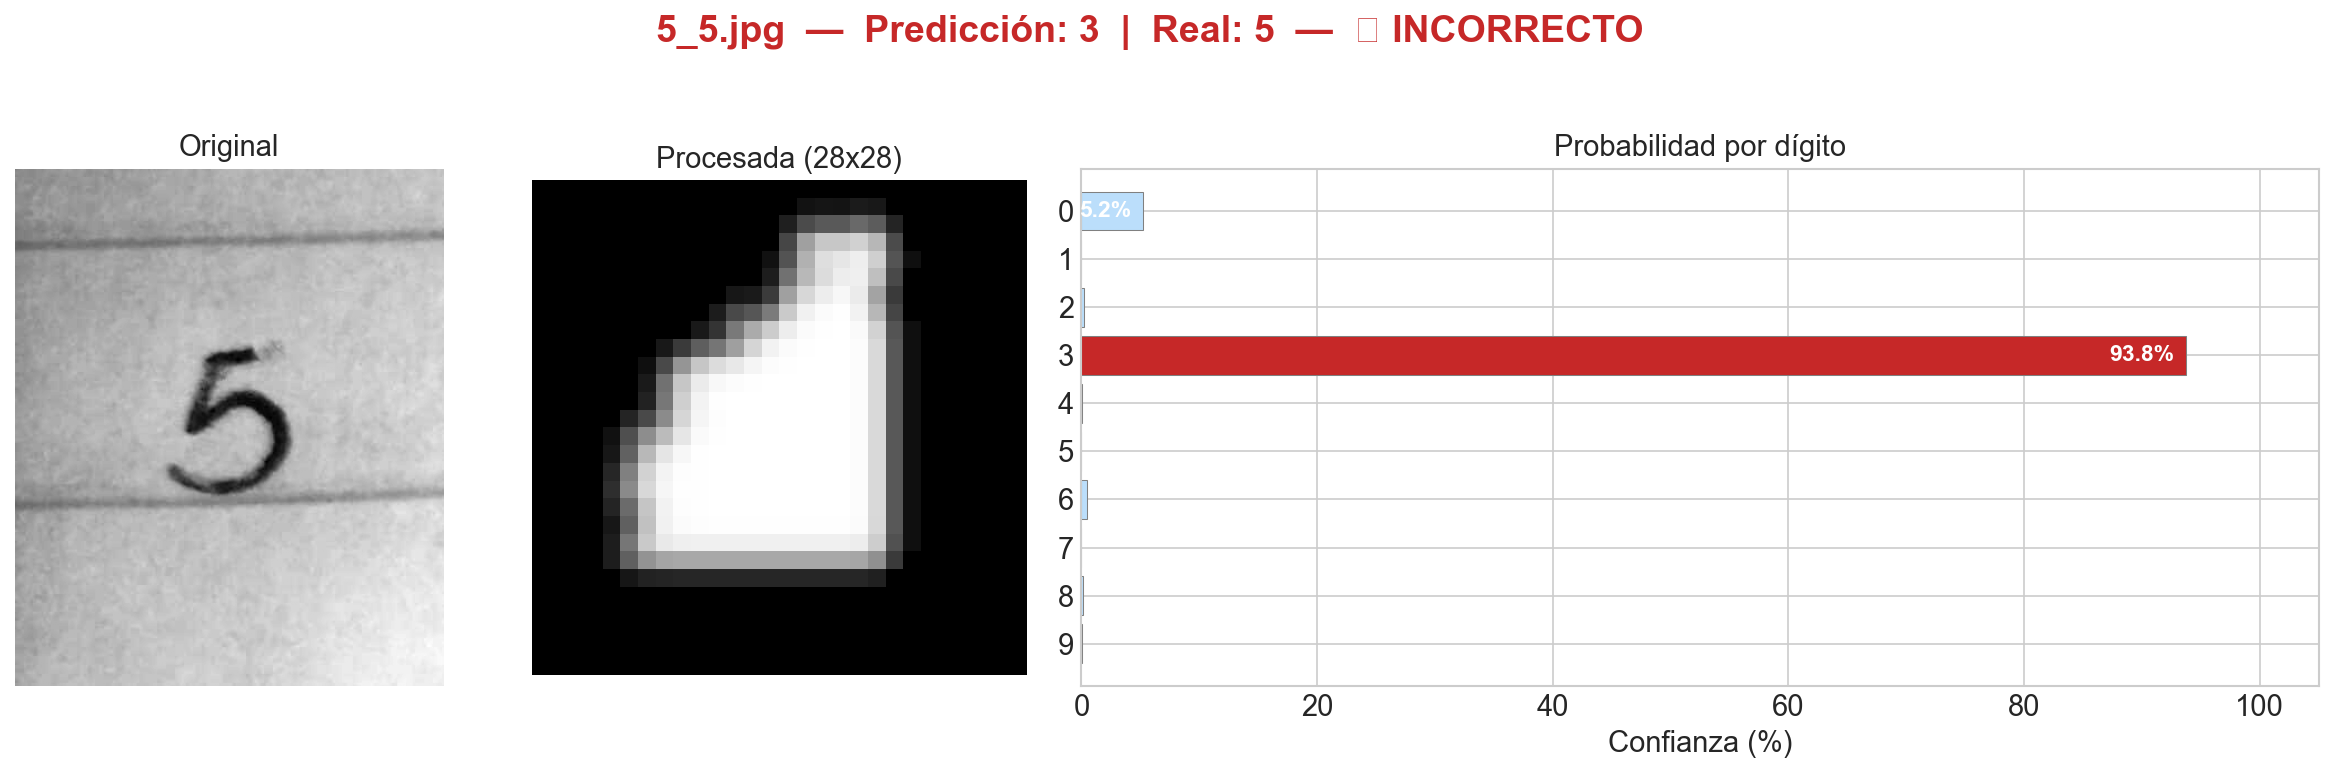
\includegraphics[width=\linewidth]{prediccion_5_5.png}
\end{center}
\end{columns}

\vspace{0.2cm}
\begin{center}
\small Fotos grandes con textura de papel $\rightarrow$ ruido residual confunde al modelo
\end{center}
\end{frame}

%========== SLIDE 11: CONFUSION PROPIAS ==========
\begin{frame}{Analisis de Errores}
\begin{columns}
\column{0.5\textwidth}
\begin{center}
    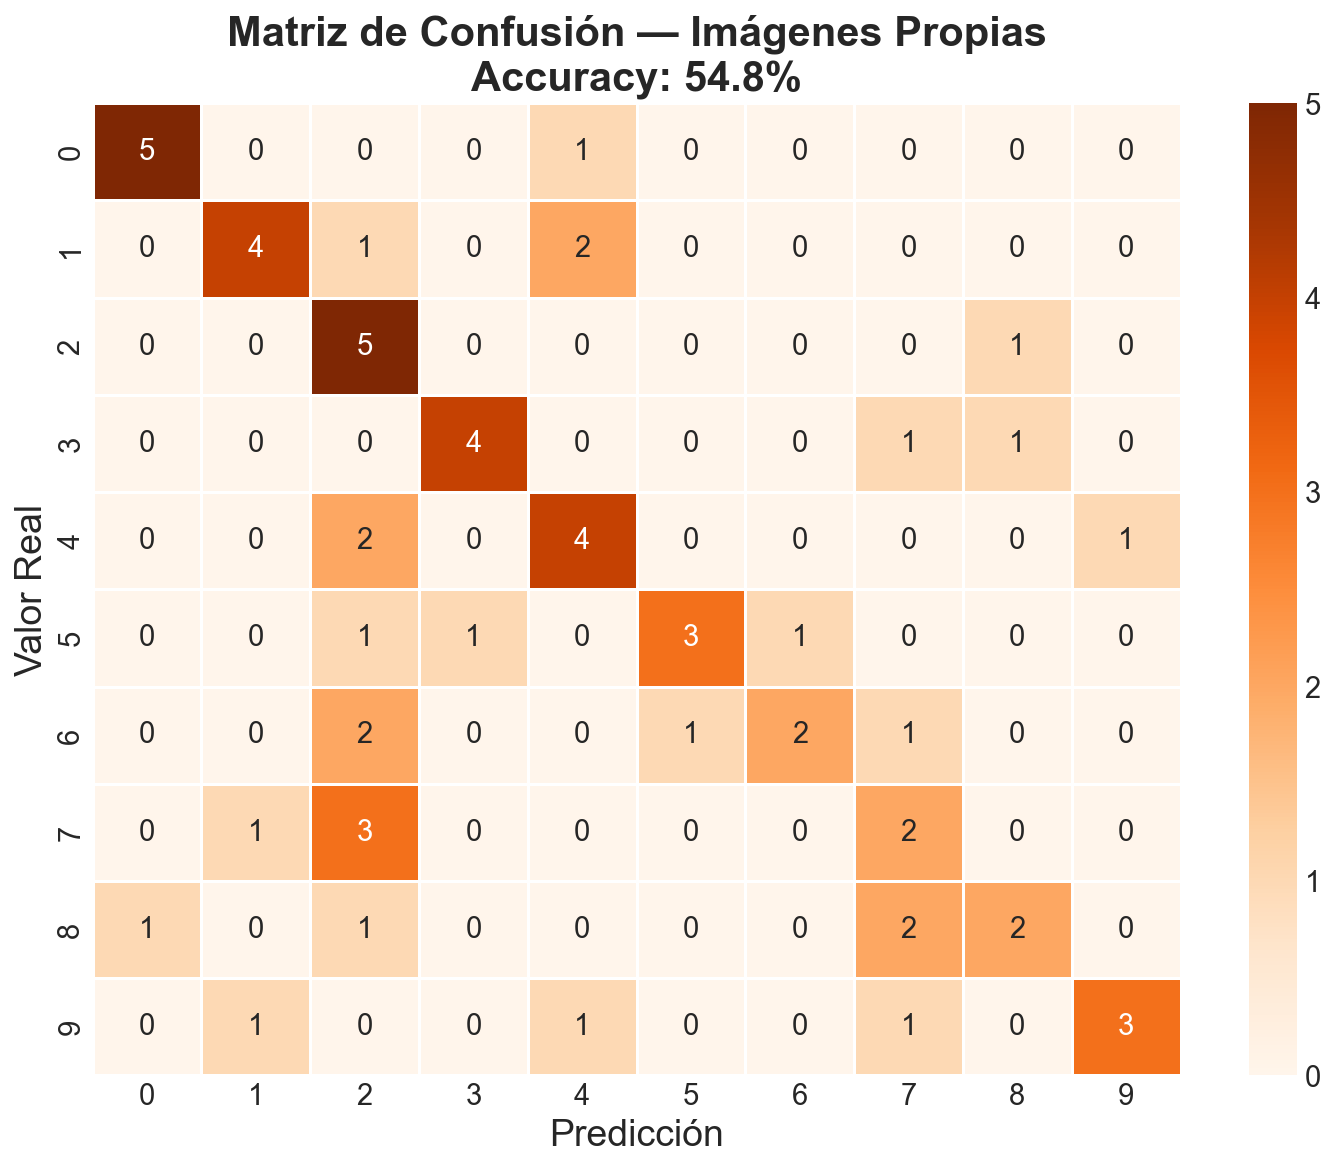
\includegraphics[width=\linewidth]{confusion_propias.png}

    \small Matriz de confusion --- imagenes propias
\end{center}

\column{0.5\textwidth}
\textbf{¿Por que baja el accuracy?}
\begin{enumerate}
    \item \textbf{Dominio diferente:} fotos de celular $\neq$ escaneos de MNIST
    \item \textbf{Textura del papel:} ruido residual que no existe en MNIST
    \item \textbf{Grosor de trazo:} marcador vs lapiz digital de MNIST
    \item \textbf{Estilo personal:} variaciones en la forma de escribir
\end{enumerate}

\vspace{0.3cm}
\textbf{Hallazgo clave:}\\
Recortes cercanos (95\%) vs fotos de pagina (33\%)\\
$\rightarrow$ La calidad de la foto importa tanto como el modelo
\end{columns}
\end{frame}

%========== SLIDE 12: CONCLUSIONES ==========
\begin{frame}{Conclusiones}
\begin{enumerate}
    \item Un \textbf{MLP con 3 capas ocultas} (256, 128, 64) logra \textbf{98.43\%} en MNIST
    \item El \textbf{data augmentation} mejora la robustez del modelo ante variaciones reales
    \item El rendimiento en imagenes propias depende fuertemente del \textbf{preprocesamiento}
    \item \textbf{Leccion clave:} un modelo es tan bueno como la \textbf{representatividad} de sus datos de entrenamiento respecto a los datos reales
\end{enumerate}

\vspace{0.4cm}
\begin{block}{Posibles mejoras}
\begin{itemize}
    \item Usar \textbf{redes convolucionales} (CNN) para capturar patrones espaciales
    \item Mejorar la captura de imagenes (fondo uniforme, recorte cercano)
    \item Fine-tuning con un subconjunto de imagenes propias
\end{itemize}
\end{block}
\end{frame}

%========== SLIDE 13: GRACIAS ==========
\begin{frame}
\begin{center}
    {\Huge ¿Preguntas?}

    \vspace{1cm}
    {\large Codigo disponible en GitHub}

    \vspace{0.3cm}
    \texttt{github.com/TUUSUARIO/mnist-handwritten-digits}
\end{center}
\end{frame}

\end{document}
